\documentclass{article}
\usepackage[utf8]{inputenc}
\usepackage[default]{raleway}
\usepackage[table]{xcolor}
\usepackage{booktabs} 
\usepackage{ragged2e}
\usepackage{subcaption}
\usepackage{pgf-pie, multirow, longtable, tikz, titlesec, comment, tabularx, makecell, float, listings, array, setspace, geometry, graphicx, xcolor, xparse, fancyvrb, relsize, fancyhdr, booktabs, hyperref, eurosym, fancybox, cleveref, todonotes}
%\geometry{a4paper, left=2cm, right=2cm, top=2cm, bottom=2.5cm}

\renewcommand{\headrulewidth}{0pt}

% ----------------------------- Definizione tabella ---------------------------

\newcolumntype{C}[1]{>{\centering\arraybackslash}m{#1}}
\newcolumntype{L}[1]{>{\RaggedRight\arraybackslash}m{#1}}

% ------------------------------Metadati indice -------------------------------

\titleformat{\paragraph}[hang]{\normalfont\normalsize\bfseries}{\theparagraph}{1em}{}
\titlespacing*{\paragraph}{0pt}{0.2cm plus 0.1cm minus 0.05cm}{0.1cm plus 0.05cm minus 0.02cm}

% ------------------------------Metadati indice -------------------------------
\title{\textbf{\fontsize{30}{6}\selectfont Indice}}
\author{\fontsize{14}{6}\selectfont ByteOps}
\date{}

% -----------------------------Creazione footer --------------------------------
\pagestyle{fancy} 
\fancyhf{}
\renewcommand{\footrulewidth}{0.4pt} 
\lfoot{ 
    \parbox[c]{2cm}{
\includegraphics[width=2cm]{../Images/logo.png}}
    \textcolor[RGB]{120, 120, 120}{$\cdot$ Manuale utente}
}
\rfoot{\thepage}
 
% --------------------------Modifica formato hyperlinks ------------------------
\hypersetup{
    colorlinks=true,
    linkcolor=darkgreen,
    urlcolor=navyblue,
    filecolor=black,      
    pdftitle={Manuale utente},
    pdfpagemode=FullScreen,
}

\definecolor{responsabile}{RGB}{0,102,204}
\definecolor{amministratore}{RGB}{0,204,102}
\definecolor{analista}{RGB}{255,165,0}
\definecolor{progettista}{RGB}{255,0,0}
\definecolor{programmatore}{RGB}{128,0,128}
\definecolor{verificatore}{RGB}{255,192,203}

\definecolor{responsabile}{RGB}{0,102,204}
\definecolor{amministratore}{RGB}{0,204,102}
\definecolor{analista}{RGB}{255,165,0}
\definecolor{progettista}{RGB}{255,0,0}
\definecolor{programmatore}{RGB}{128,0,128}
\definecolor{verificatore}{RGB}{255,192,203}

\definecolor{darkgreen}{rgb}{0.0, 0.5, 0.0}
\definecolor{navyblue}{rgb}{0.0, 0.0, 0.8}


\begin{document}
\pagestyle{fancy}
\begin{center}
    
\includegraphics[width = 0.7\textwidth]{../Images/logo.png} \\
    \vspace{0.2cm}
    \textcolor[RGB]{60, 60, 60}{\textit{ByteOps.swe@gmail.com}} \\
    \vspace{1cm}
    \fontsize{16}{6}\selectfont Manuale utente \\
    \vspace{0.5cm}
\end{center}

\section*{Informazioni documento}
\def\arraystretch{1.2}
\begin{tabular}{>{\raggedleft\arraybackslash}p{0.2\textwidth}|>{\raggedright\arraybackslash}p{0.6\textwidth}c}
    \hline
    \addlinespace
    \textbf{Redattori}    & A. Barutta\\ & R. Smanio\\ & L. Skenderi\\ & F. Pozza\\ & D. Diotto \\ & N. Preto \vspace{10pt} \\
    \textbf{Verificatori} & E. Hysa\\ & A. Barutta\\ & D. Diotto\\ & L. Skenderi\\ & R. Smanio\\ & F. Pozza \vspace{10pt} \\
    \textbf{Destinatari}  & ByteOps\\ & T. Vardanega   \\ & R. Cardin \vspace{10pt} \\
\end{tabular}
\pagebreak

% ------------------------- Changelog ----------------------------
\section*{Registro delle modifiche}
\begin{tabular}{|C{1.5cm}|C{2.1cm}|C{2cm}|C{2cm}|C{4.5cm}|}
    \hline 
    \textbf{Versione} & \textbf{Data} & \textbf{Autore} & \textbf{Verificatore} & \textbf{Dettaglio} \\
    \hline
    \label{Git_Action_Version} 1.0.0 & 25/03/2024 & A. Barutta & D. Diotto & Correzioni finali  \\
    \hline 0.2.5 & 09/03/2024 & L. Skenderi & D. Diotto & Correzioni changelog  \\
    \hline
    0.2.4 & 08/03/2024 & F. Pozza & A. Barutta & Correzione riferimenti  \\
    \hline
    0.2.3 & 04/03/2024 & N. Preto & A. Barutta & Aggiunta sotto-sezione Gruppi pannelli in dettaglio  \\
    \hline
    0.2.2 & 02/03/2024 & N. Preto & F. Pozza & Completamento sotto-sezione Alert \\
    \hline
    0.2.1 & 01/03/2024 & D. Diotto & E. Hysa & Aggiunta sotto-sezione Alert \\
    \hline
    0.2.0 & 29/02/2024 & R. Smanio & N. Preto & Aggiunta sezione Requisiti \\
    \hline
    0.1.4 & 25/02/2024 & D. Diotto & N. Preto & Modifica formattazione immagini \\
    \hline
    0.1.3 & 22/02/2024 & A. Barutta & F. Pozza & Stesura sotto-sezione Dashboard dettagliate \\
    \hline
    0.1.2 & 20/02/2024 & A. Barutta & F. Pozza & Stesura sotto-sezione Profilo utente \\
    \hline
    0.1.1 & 20/02/2024 & L. Skenderi & R. Smanio & Modifica sezione Istruzioni all'uso \\
    \hline
    0.1.0 & 16/02/2024 & L. Skenderi & A. Barutta & Aggiunta sezione Istruzioni all'uso \\
    \hline
    0.0.1 & 13/02/2024 & D. Diotto & A. Barutta & Impostazione generale \\ 
    \hline
\end{tabular}

\pagebreak

% ------------------------- Generazione automatica indice ----------------------
\setstretch{1.5}
\maketitle
\thispagestyle{fancy}
{
    \hypersetup{linkcolor=black}
    \tableofcontents
    \setcounter{tocdepth}{4}
    \listoffigures
    \listoftables 
}
\setstretch{1.2}
\pagebreak

% ---------------------------- Inizio documento -------------------------------

\flushleft

\section{Introduzione}

\subsection{Scopo del Manuale}
Il manuale ha lo scopo di assistere l’utente passo dopo passo per un corretto utilizzo del
software così da sfruttarne appieno tutte le funzionalità presenti per offrire un’esperienza
ottimale

\subsection{Glossario}
Incluso nella documentazione è presente il \textbf{\textit{Glossario}} in cui sono definiti tutti i termini specifici o eventualmente ambigui presenti nei vari documenti del progetto. Se un termine è nel \textbf{\textit{Glossario}}, viene segnalato con una \textit{G} a pedice accanto ad esso.

\subsubsection{Raccolta termini del glossario}
Il \textbf{\textit{Glossario}} verrà compilato attraverso un documento condiviso su \LaTeX \textsubscript{\textit{G}}, accessibile a ttti i membri del gruppo. Qui, verranno elencati i ter min  i di particolare rilevanza nel contesto del progetto, seguendo una checklist.   Successivamente, l'\textit{Amministratore} del progetto si occuperà di dettagliare  ulteriormente questi termini nella creazione del \textbf{\textit{Glossario}} ufficiale. 
\subsection{Riferimenti}
\subsubsection{Riferimenti informativi}
    \begin{itemize}
        \item \href {https://www.math.unipd.it/~tullio/IS-1/2023/Progetto/C6.pdf} {Capitolato d'appalto C6 - InnovaCity }
        \item \href{https://www.math.unipd.it/~tullio/IS-1/2023/Dispense/T4.pdf} {Slide del corso di Ingegneria del Software - Gestione di progetto }
        \item \href{https://www.math.unipd.it/~tullio/IS-1/2023/Dispense/T2.pdf} {Slide del corso di Ingegneria del Software - Ciclo di vita del software }
    \end{itemize}
 
\subsubsection{Riferimenti normativi}
    \begin{itemize}
    \item Norme di progetto
    \item \href {https://www.math.unipd.it/~tullio/IS-1/2023/Dispense/PD2.pdf} {Regolamento del progetto didattico }
    \end{itemize}

\vspace{0.5cm}

\section{Requisiti}
Per poter utilizzare il software occorre rispettare i seguenti
requisiti minimi:  

\subsection{Requisiti hardware}
L’applicazione esegue su \textit{browser}\textsubscript{\textit{G}}, come tale non si individuano dei requisiti specifici, fissati da parte
della \textit{proponente}\textsubscript{\textit{G}}, dal capitolato o dal progetto stesso. I seguenti, pertanto, sono individuati come
riferimento di massima per l’esecuzione del prodotto creato.   
\begin{table}[H]
    \centering
    \begin{tabular}{ll}
        \toprule
        \textbf{Componente} & \textbf{Requisito} \\
        \midrule
        Processore & \textit{Dual-core CPU}\textsubscript{\textit{G}}, \textit{clock rate}\textsubscript{\textit{G}}: 1.5 GHz \\
        Memoria & 2 GB di RAM \\
        Spazio su disco & 10 GB di spazio disponibile\\
        \bottomrule
    \end{tabular}
    \caption{Requisiti hardware minimi}
\end{table} 
\subsubsection{Requisiti software}
Di seguito sono elencati i \textit{browser}\textsubscript{\textit{G}} per i quali è garantita la compatibilità con il dispositivo (desktop o mobile). È importante notare che l'applicazione potrebbe funzionare anche su altri \textit{browser}\textsubscript{\textit{G}} o versioni precedenti, ma non è garantito il pieno supporto.  
\begin{table}[H]
    \centering
    \begin{tabular}{ll}
        \toprule
        \textbf{Browser} & \textbf{Versione} \\
        \midrule
        \textit{Chrome}\textsubscript{\textit{G}} & v.89.0.4389.82\\
        \textit{Firefox}\textsubscript{\textit{G}} & v.86.0 \\
        \textit{Safari}\textsubscript{\textit{G}} & v.14.0 \\
        \textit{Edge}\textsubscript{\textit{G}} & v.89.0.774.54 \\
        \bottomrule
    \end{tabular}
    \caption{Browser e versioni supportate}
\end{table}

Inoltre, vengono indicate le versioni minime dei sistemi operativi necessarie per poter utilizzare l'applicazione. Come avviene per i \textit{browser}\textsubscript{\textit{G}}, l'applicazione potrebbe operare su sistemi operativi differenti o su versioni precedenti, tuttavia, non è garantito il completo supporto.\\
\begin{table}[H]
    \centering
    \begin{tabular}{ll}
        \toprule
        \textbf{OS} & \textbf{Versione} \\
        \midrule
        \textit{Linux}\textsubscript{\textit{G}} & Ubuntu: versione 18.04 LTS\\&Debian: versione 9\\& RHEL: versione 7\\& CentOS: versione 7\\& Fedora: versione 30 \\
        \textit{Windows}\textsubscript{\textit{G}} & \textit{Windows}\textsubscript{\textit{G}} 10, \textit{Windows}\textsubscript{\textit{G}} Server 2012 R2 \\
        \textit{MacOS}\textsubscript{\textit{G}} & macOS 10.13 (High Sierra) \\
        \bottomrule
    \end{tabular}
    \caption{Sistemi operativi e versioni supportate}
\end{table} 

\section{Istruzioni all'uso}
\subsection{Login}

All'avvio il sito presenta una schermata di accesso, in cui gli utenti sono invitati a inserire le proprie credenziali fornite dagli amministratori (username e password) per ottenere l'accesso al sistema. Si precisa che solo gli utenti autorizzati hanno il permesso di accedere al servizio. Dopo aver compilato correttamente i campi richiesti, l'utente può procedere cliccando sul pulsante di Login, il quale lo reindirizzerà alla dashboard principale del sistema. \\
\begin{figure}[H]
    \centering
    \fbox{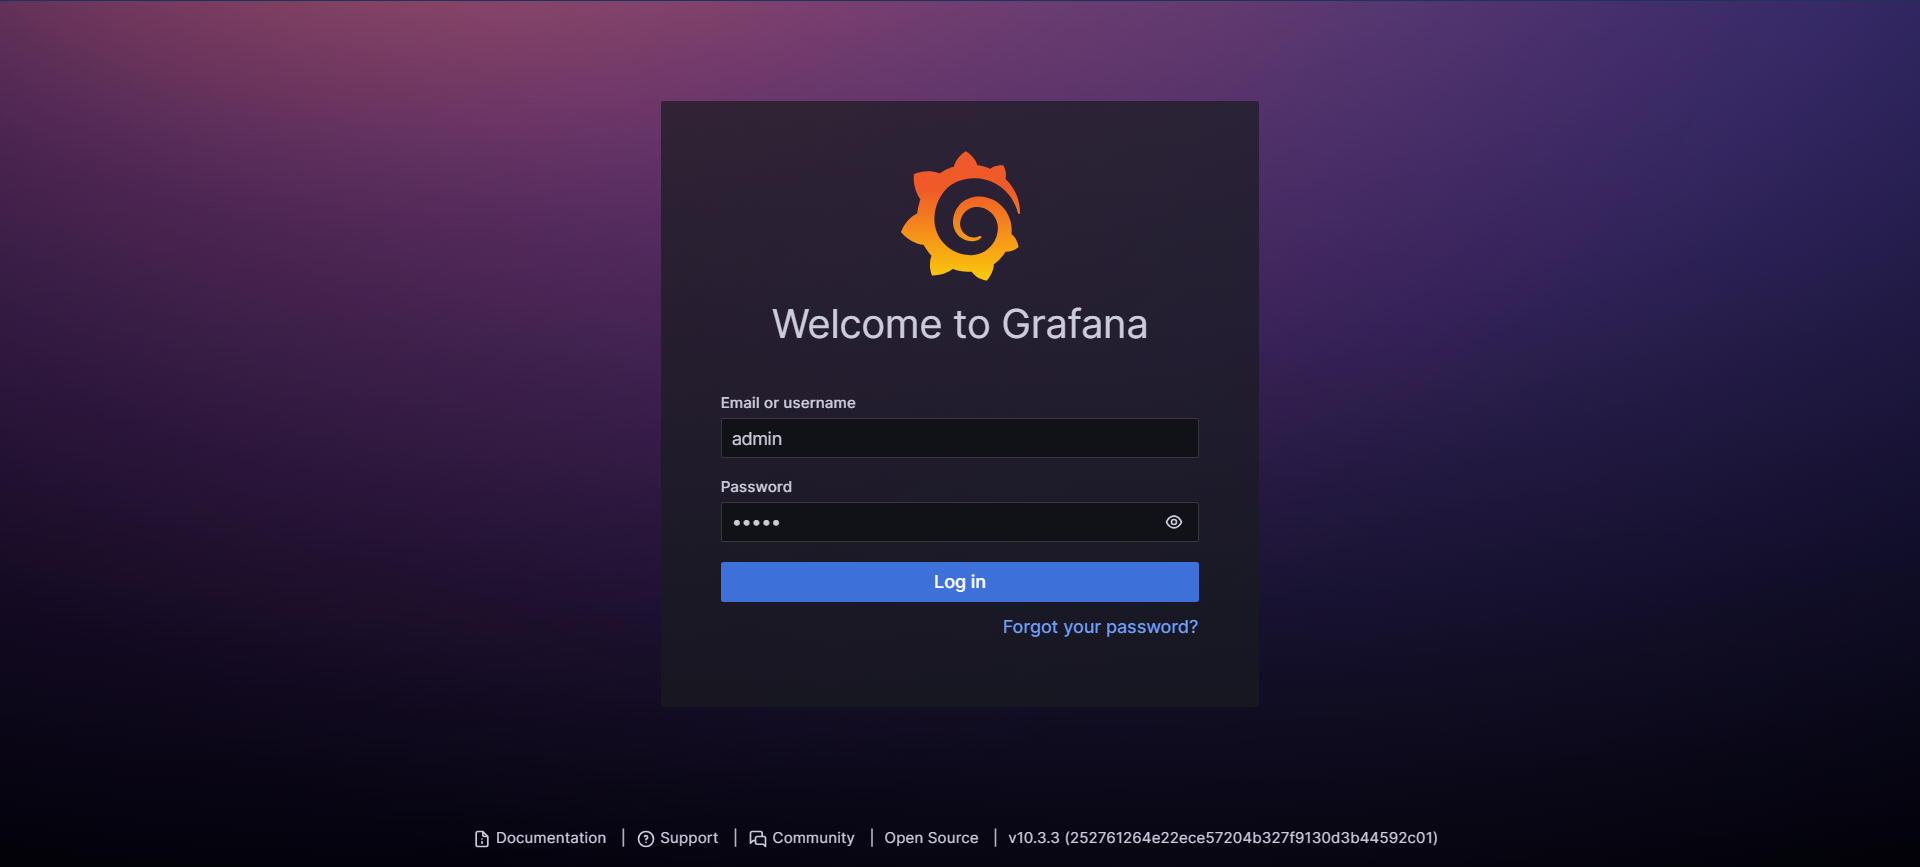
\includegraphics[width=13cm]{../Images/ManualeUtente/login.png}}
    \caption{Schermata di accesso al sistema}
    \label{fig:my_label}
\end{figure}
Nel caso in cui le credenziali siano errate, il sistema mostrerà un messaggio di errore all’utente:\\
\begin{figure}[H]
    \centering
    \fbox{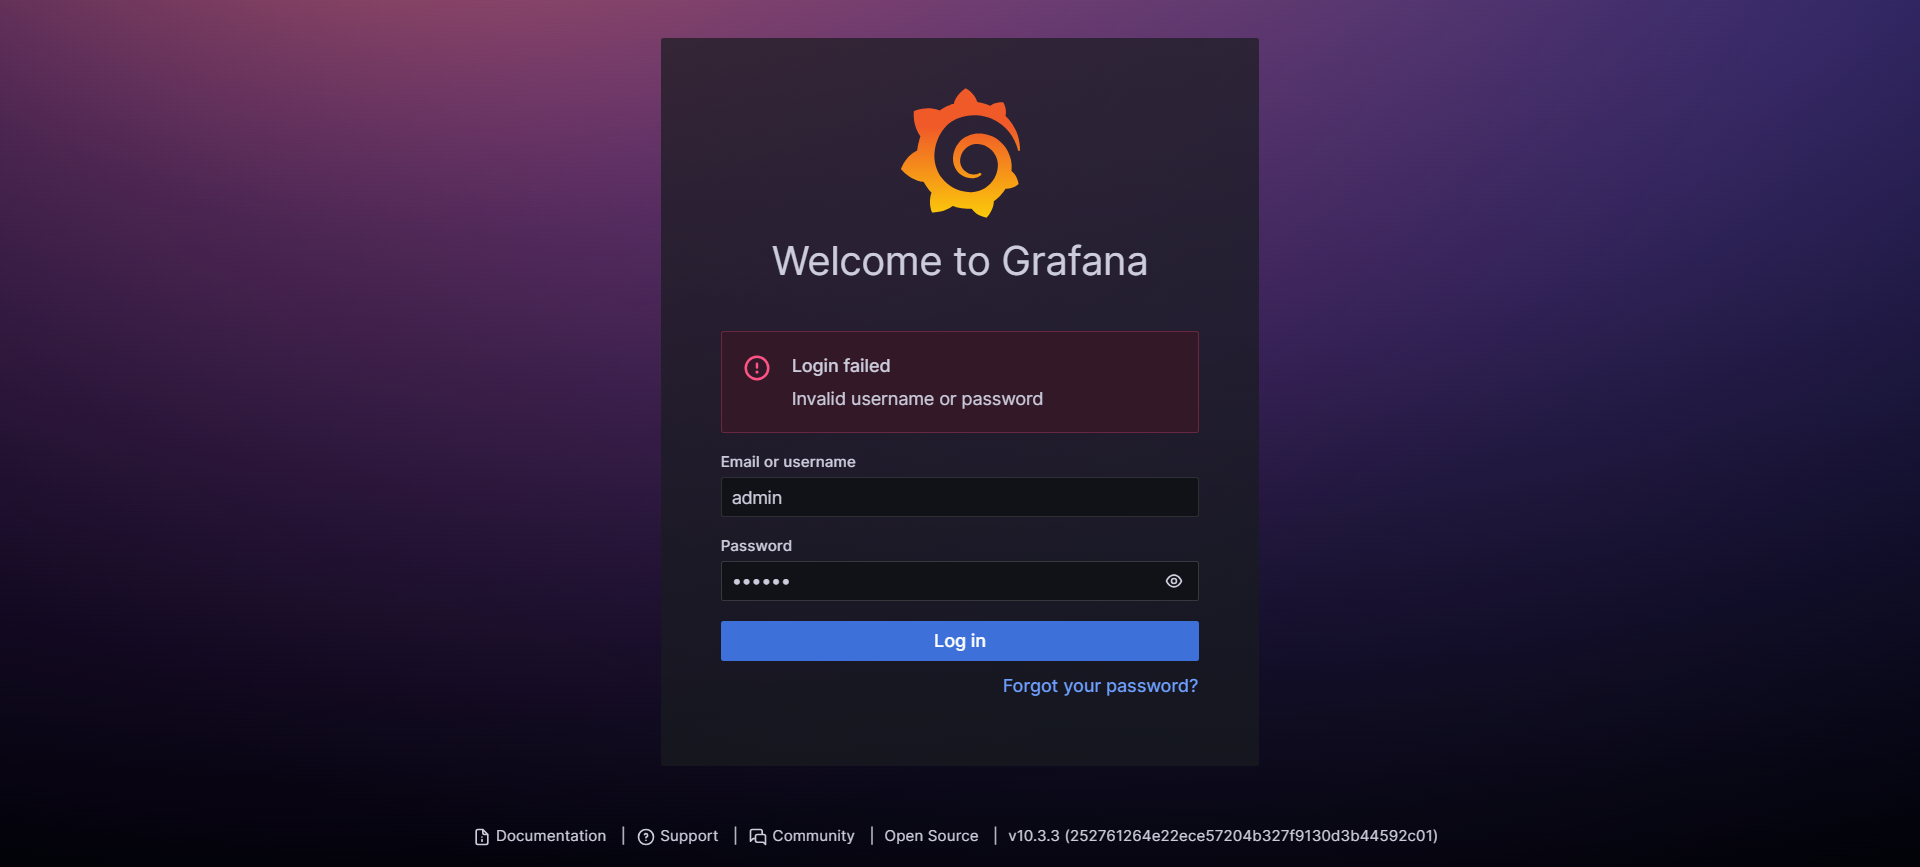
\includegraphics[width=13cm]{../Images/ManualeUtente/login-error-username_wide.png}}
    \caption{Messaggio di errore per username errato}
    \label{fig:my_label}
\end{figure}
\subsection{Dashboard}
Una \textit{dashboard}\textsubscript{\textit{G}} costituisce il cruscotto di controllo primario del \textit{sistema}\textsubscript{\textit{G}}, rappresentando una composizione di diversi pannelli che visualizzano i dati in tempo reale provenienti dai sensori. \\
Ogni pannello consente la visualizzazione dei dati in modo appropriato, adottando grafici di diversa natura in base alla tipologia di informazioni. Ad esempio, nel caso di dati temporali, il pannello mostrerà un grafico a linee, mentre per la visualizzazione di dati spaziali, sarà presentata una mappa interattiva che illustra la posizione, la tipologia e le misurazioni dei sensori.\\
Per ciascun gruppo di pannelli, saranno inclusi anche valori numerici contenenti informazioni aggiuntive e specifiche. Questi valori mostreranno aggregazioni dei dati, la disponibilità di risorse specifiche o il punteggio di salute complessivo della città. \\
\begin{figure}[H]
    \centering
    \fbox{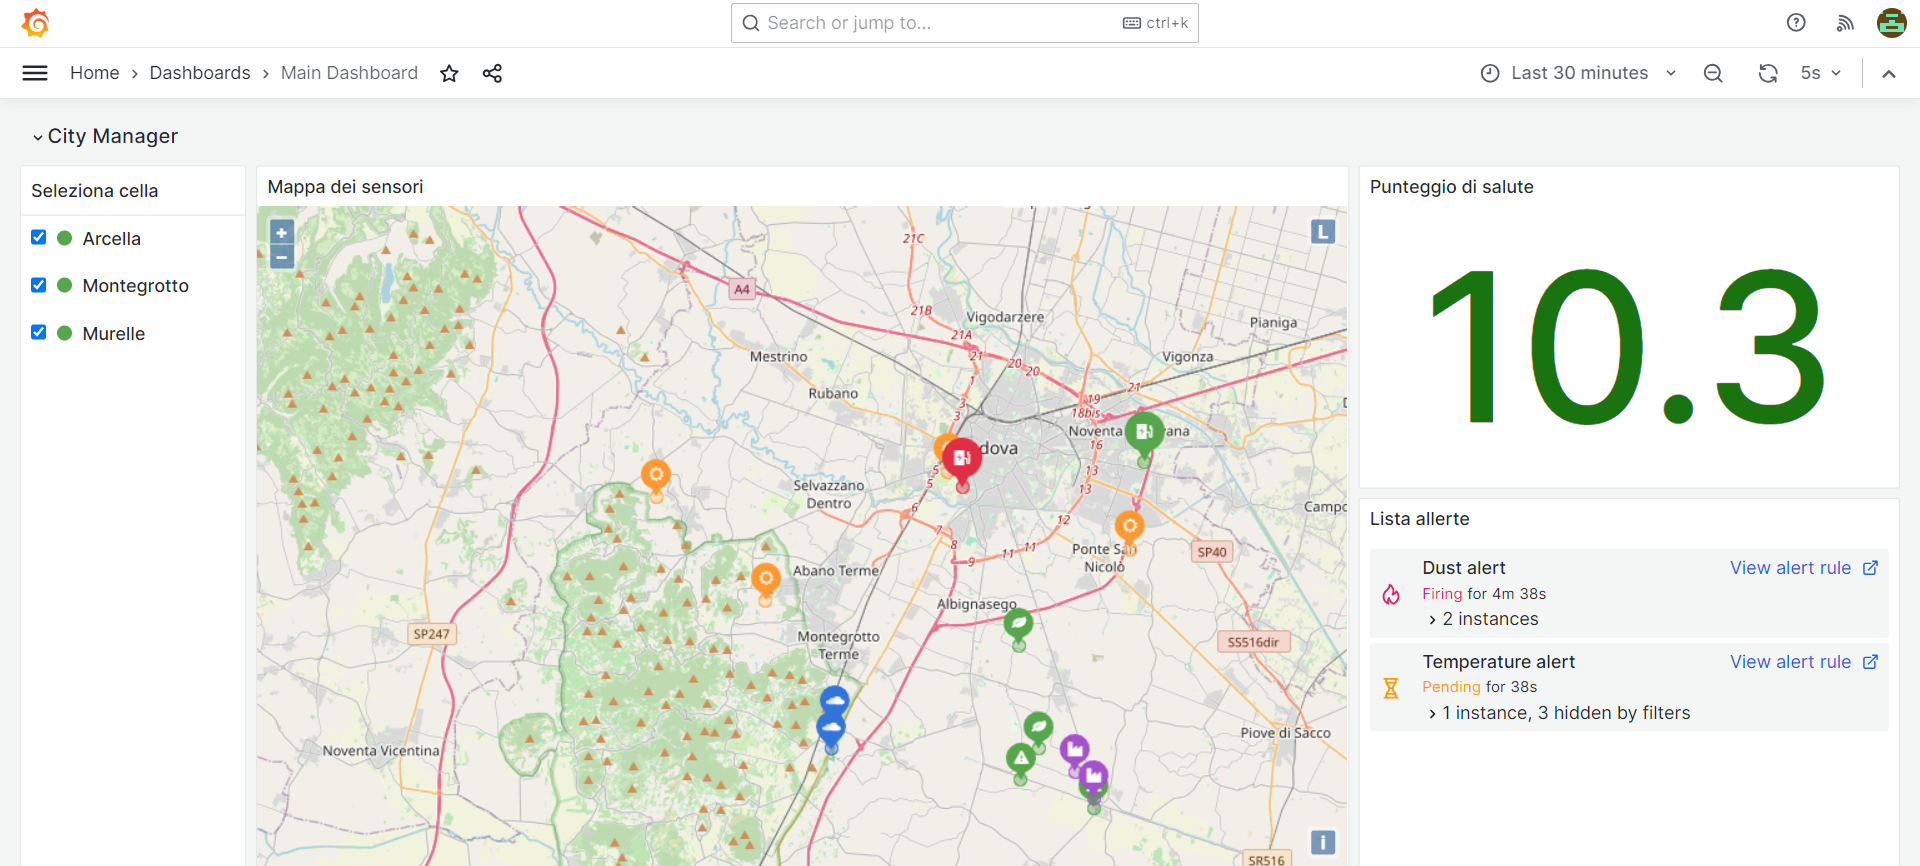
\includegraphics[width=16cm]{../Images/ManualeUtente/Light/dashboard_principale_light_alert.png}}
    \caption{Esempio di dashboard principale}
    \label{fig:my_label}
\end{figure}


\subsubsection{Barra degli strumenti}
\label{sec:barra_strumenti}
La barra degli strumenti è una sezione della \textit{dashboard}\textsubscript{\textit{G}} posizionata nella parte superiore della pagina. Essa fornisce una serie di pulsanti, icone e menu a tendina che consentono agli utenti di eseguire azioni specifiche o di accedere a funzionalità aggiuntive in modo rapido e intuitivo. \\
\begin{figure}[H]
    \centering
    \fbox{
\includegraphics[width=16cm]{../Images/ManualeUtente/Light/toolbar.png}}
    \caption{Barra degli strumenti}
    \label{fig:my_label}
\end{figure}

\paragraph{Pulsante profilo utente}
\hypertarget{par:pulsante_profilo}{}
Il pulsante del profilo utente consente all'utente di accedere al proprio profilo personale, dove potrà visualizzare e modificare le proprie informazioni personali, le impostazioni dell'\textit{account}\textsubscript{\textit{G}} e le preferenze. \\
Una volta premuto il pulsante, verrà visualizzato un menu a tendina con le seguenti opzioni:
\begin{itemize}
    \item Profile: permette di visualizzare e modificare le informazioni personali;
    \item Notification history: consente di visualizzare la cronologia delle notifiche ricevute;
    \item Change password: offre la possibilità di modificare la password dell'\textit{account}\textsubscript{\textit{G}};
    \item Sign out: permette di effettuare il \textit{logout}\textsubscript{\textit{G}} dal \textit{sistema}\textsubscript{\textit{G}}.
\end{itemize}
\begin{figure}[H]
    \centering
    \fbox{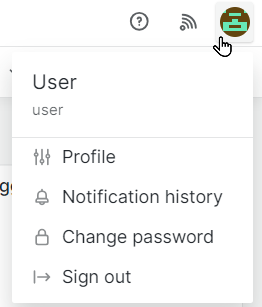
\includegraphics[width=5cm]{../Images/ManualeUtente/Light/toolbar_dettaglio_user.png}}
    \caption{Pulsante profilo utente}
    \label{fig:my_label}
\end{figure}


\paragraph{Barra di ricerca}
La barra di ricerca consente all'utente di cercare e filtrare le \textit{dashboard}\textsubscript{\textit{G}} disponibili o di cambiare pagina. L'utente può digitare il nome della \textit{dashboard}\textsubscript{\textit{G}} o della pagina desiderata e premere "Invio" per visualizzare i risultati della ricerca.  
\begin{figure}[H]
    \centering
    \fbox{
\includegraphics[width=7cm]{../Images/ManualeUtente/Light/toolbar_dettaglio_navbar.png}}
    \caption{Barra di ricerca}
    \label{fig:my_label}
\end{figure}

\paragraph{Menu ad hamburger}
Il menu ad hamburger è un'icona costituita da tre linee orizzontali sovrapposte, che rappresenta un pulsante per l'apertura di un menu a discesa. Questo menu consente all'utente di accedere a funzionalità aggiuntive. \\
Queste funzionalità sono:
\begin{itemize}
    \item Home: offre la possibilità di tornare alla homepage di \textit{Grafana}\textsubscript{\textit{G}};
    \item Starred: permette di visualizzare le \textit{dashboard}\textsubscript{\textit{G}} preferite;
    \item Dashboards: consente di accedere alla lista delle \textit{dashboard}\textsubscript{\textit{G}} disponibili;
    \item Alerting: offre la possibilità di visualizzare ed esportare le regole di allerta e notifiche;
\end{itemize}
\begin{figure}[H]
    \centering
    \fbox{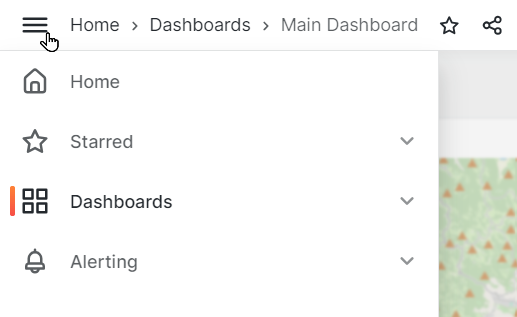
\includegraphics[width=9cm]{../Images/ManualeUtente/Light/toolbar_dettaglio_hamburger.png}}
    \caption{Menu ad hamburger}
    \label{fig:my_label}
\end{figure}

\paragraph{Breadcrumb}
Il breadcrumb è composto da una serie di \textit{link}\textsubscript{\textit{G}} che mostrano la posizione corrente dell'utente all'interno del sito. Questi \textit{link}\textsubscript{\textit{G}} consentono all'utente di navigare facilmente all'interno del sito, tornando indietro o spostandosi avanti nella gerarchia delle pagine. \\
\begin{figure}[H]
    \centering
    \fbox{
\includegraphics[width=7cm]{../Images/ManualeUtente/Light/toolbar_dettaglio_breadcrumb.png}}
    \caption{Breadcrumb}
    \label{fig:my_label}
\end{figure} 

\paragraph{Mark as favorite}
Il pulsante "Mark as favorire", letteralmente "Segna come preferita", è un pulsante che permette di segnare una \textit{dashboard}\textsubscript{\textit{G}} come "preferita" e di accedervi con maggiore facilità.
\begin{figure}[H]
    \centering
    \fbox{
\includegraphics[width=7cm]{../Images/ManualeUtente/Light/toolbar_dettaglio_star.png}}
    \caption{Pulsante "Mark as favorite"}
    \label{fig:my_label}
\end{figure}

\paragraph{Share}
Il pulsante "Share" permette di condividere con altri utenti la \textit{dashboard}\textsubscript{\textit{G}} attualmente aperta. Una volta premuto il pulsante offrirà all'utente una serie di opzioni per configurare al meglio la condivisione, tra cui: 
\begin{itemize}
    \item generare e configurare un \textit{link}\textsubscript{\textit{G}} per la condivisione;
    % NOTA: \textit{Snapshot}\textsubscript{\textit{G}} finisce nel glossario
    \item generare uno \textit{snapshot}\textsubscript{\textit{G}} della \textit{dashboard}\textsubscript{\textit{G}} attuale;
    \item esportare la \textit{dashboard}\textsubscript{\textit{G}} come file;
    \item pubblicare la \textit{dashboard}\textsubscript{\textit{G}}.
\end{itemize}
\begin{figure}[H]
    \centering
    \fbox{
\includegraphics[width=7cm]{../Images/ManualeUtente/Light/toolbar_dettaglio_share.png}}
    \caption{Pulsante "Share"}
    \label{fig:my_label}
\end{figure}

\paragraph{Intervallo temporale}
Il menu a tendina "Intervallo temporale" permette all'utente di selezionare l'intervallo temporale desiderato per la visualizzazione dei dati. La \textit{dashboard}\textsubscript{\textit{G}} offre una serie di intervalli predefiniti e, inoltre, permette all'utente di personalizzarli secondo le proprie necessità. \\
Eventuali aggregazioni delle misurazioni o operazioni effettuate sui dati verranno applicate in base all'intervallo temporale selezionato.
\begin{figure}[H]
    \centering
    \fbox{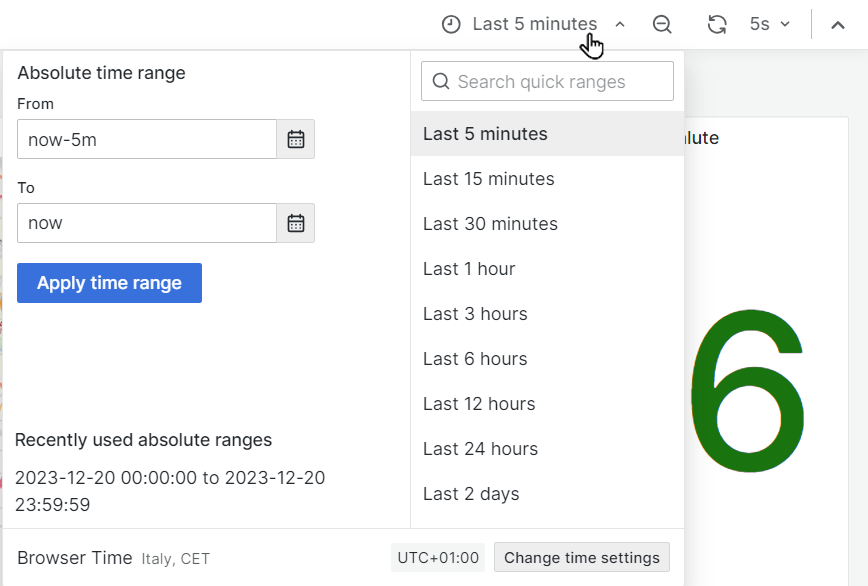
\includegraphics[width=7cm]{../Images/ManualeUtente/Light/toolbar_dettaglio_timerange.png}}
    \caption{Menu "Intervallo temporale"}
    \label{fig:my_label}
\end{figure}

\paragraph{Zoom out}
Il pulsante "Zoom out" consente all'utente di regolare la visualizzazione dei grafici per mostrare un intervallo temporale più ampio, secondo intervalli temporali predefiniti. 
\begin{figure}[H]
    \centering
    \fbox{
\includegraphics[width=7cm]{../Images/ManualeUtente/Light/toolbar_dettaglio_zoomout.png}}
    \caption{Pulsante "Zoom out"}
    \label{fig:my_label}
\end{figure}

\paragraph{Ricarica dashboard}
Il pulsante "Ricarica \textit{dashboard}\textsubscript{\textit{G}}" permette all'utente di aggiornare la \textit{dashboard}\textsubscript{\textit{G}} attuale per visualizzare i dati più recenti.  Inoltre, offre un menu a tendina attraverso il quale l'utente può impostare la frequenza di aggiornamento automatico della \textit{dashboard}\textsubscript{\textit{G}} o disattivarlo, se necessario.  
\begin{figure}[H]
    \centering
    \fbox{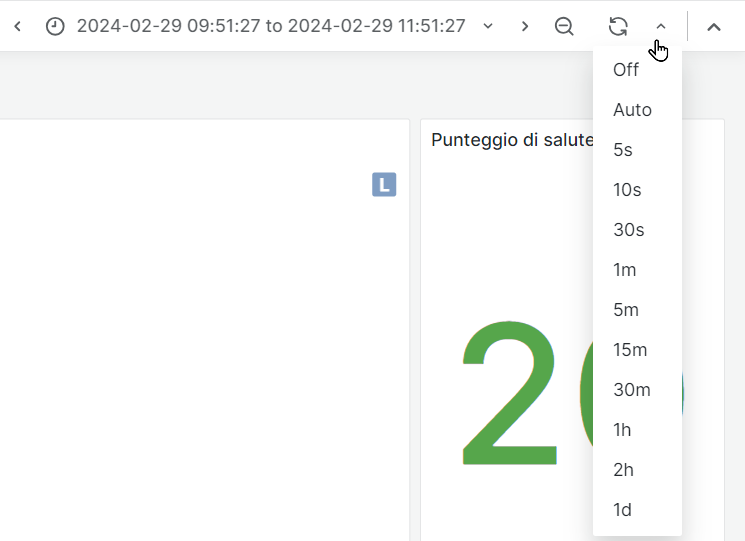
\includegraphics[width=8.5cm]{../Images/ManualeUtente/Light/toolbar_dettaglio_refresh.png}}
    \caption{Pulsante "Ricarica dashboard"}
    \label{fig:my_label}
\end{figure}

\subsubsection{Pannelli}
I pannelli costituiscono la parte principale della \textit{dashboard}\textsubscript{\textit{G}}, mostrando i dati in modo interattivo. Ogni pannello è un \textit{widget}\textsubscript{\textit{G}} progettato per visualizzare un tipo specifico di dati, adottando grafici di diversa natura in base alla tipologia di informazioni. \\
Ogni pannello contiene delle informazioni specifiche del grafico che rappresenta come ad esempio:
\begin{itemize}
    \item il nome pannello;
    \item una breve descrizione del pannello (se presente);
    \item una legenda del grafico (se presente);
    \item un menù a tendina per la selezione delle opzioni del grafico;
    \item visualizzazione dei dati misurati.
\end{itemize}

\paragraph{Descrizione del pannello}
La descrizione del pannello è una breve spiegazione del contenuto del pannello, che può essere visualizzata cliccando sull'icona "i" posta in alto a sinistra del pannello.  
\begin{figure}[H]
    \centering
    \fbox{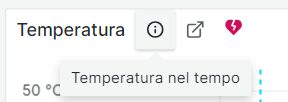
\includegraphics[width=5cm]{../Images/ManualeUtente/Light/descrizione_panel.png}}
    \caption{Descrizione del pannello}
    \label{fig:my_label}
\end{figure}

\paragraph{Legenda del grafico}
La legenda del grafico è una sezione del pannello che mostra la chiave di lettura dei dati visualizzati nel grafico. Questa sezione è utile per comprendere il significato dei colori e delle forme utilizzate nel grafico. \\
Inoltre, tramite la legenda, gli utenti possono interagire direttamente con il grafico. Ad esempio, è possibile isolare le informazioni relative a uno specifico \textit{sensore}\textsubscript{\textit{G}}. Facendo clic sul nome del \textit{sensore}\textsubscript{\textit{G}} d'interesse nella legenda del grafico, gli utenti possono concentrarsi esclusivamente sull'andamento del singolo \textit{sensore}\textsubscript{\textit{G}} selezionato. Per tornare alla visualizzazione originale, è sufficiente cliccare nuovamente sul nome del \textit{sensore}\textsubscript{\textit{G}} nella legenda.
\begin{figure}[H]
    \centering
    \fbox{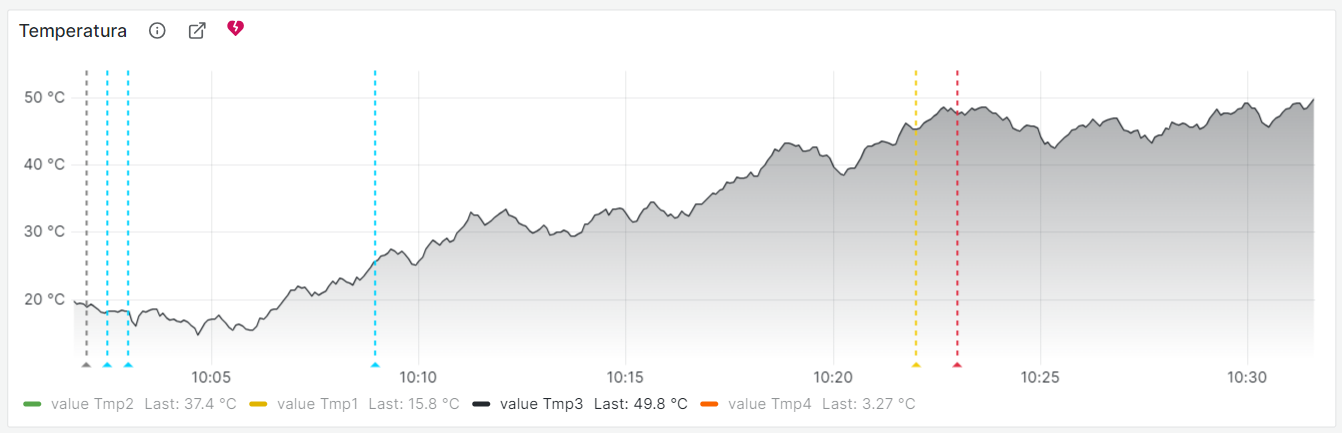
\includegraphics[width=12cm]{../Images/ManualeUtente/Light/panel_singolo_grafico.png}}
    \caption{Visualizzazione del grafico con la misurazione isolata}
    \label{fig:my_label}
\end{figure}
É inoltre possibile cambiare il colore dell'andamento di una misurazione nel grafico cliccando sul colore corrispondente nella legenda.
\begin{figure}[H]
    \centering
    \fbox{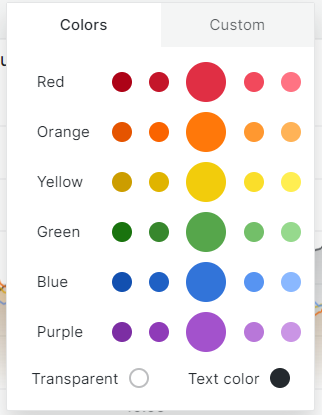
\includegraphics[width=3.5cm]{../Images/ManualeUtente/Light/colori_panel.png}}
    \caption{Cambiare il colore del grafico}
    \label{fig:my_label}
\end{figure}


\paragraph{Opzioni del pannello}
Tramite il menù a tendina delle opzioni del pannello, l'utente può accedere a diverse funzionalità aggiuntive, tra cui:
\begin{itemize}
    \item visualizzare il singolo pannello a schermo intero;
    \item condividere il pannello con altri utenti o esportarlo come file;
    \item ispezionare i dati delle misurazioni del grafico o l'intero pannello in formato JSON;
    \item nascondere o visualizzare la legenda (se presente).
\end{itemize}
\begin{figure}[H]
    \centering
    \fbox{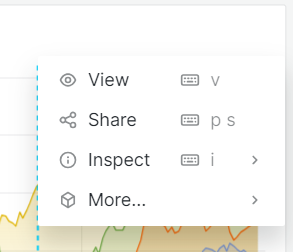
\includegraphics[width=5cm]{../Images/ManualeUtente/Light/panel_options.png}}
    \caption{Opzioni del pannello}
    \label{fig:my_label}
\end{figure}


\subsubsection{Tipologie dei grafici}
\label{subsec:tipologie_grafici}

\paragraph{Mappa sensori}
\hypertarget{par:mappa_sensori}{}
Ogni \textit{sensore}\textsubscript{\textit{G}} rappresentato sulla mappa è identificato da un pin colorato, il quale visualizza la tipologia di \textit{sensore}\textsubscript{\textit{G}} installato mediante un'icona esemplificativa. La colorazione del pin può variare in base alla tipologia di \textit{sensore}\textsubscript{\textit{G}} e alle condizioni della misurazione; ad esempio, per i sensori di rilevamento dei guasti elettrici, il pin potrebbe assumere una colorazione rossa o verde a seconda della situazione.  

Cliccando su un pin, gli utenti possono accedere alle informazioni dettagliate relative al \textit{sensore}\textsubscript{\textit{G}} specifico selezionato.
\begin{figure}[H]
    \centering
    \fbox{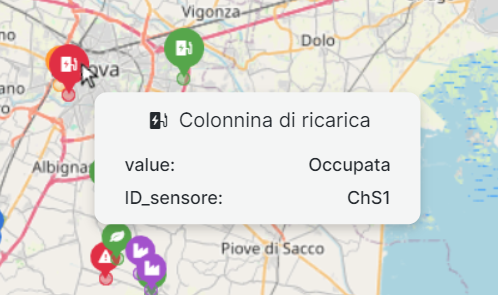
\includegraphics[width=8cm]{../Images/ManualeUtente/Light/dettaglio_mappa_light2.png}}
    \caption{Mappa sensori}
    \label{fig:my_label}
\end{figure}


\paragraph{Grafico a linee}
\hypertarget{par:grafico_linee}{}
I grafici a linee rappresentano l'andamento delle misurazioni ottenute dai sensori nel tempo. Ogni linea del grafico corrisponde a un \textit{sensore}\textsubscript{\textit{G}}, e il suo colore è associato in modo univoco ad un determinato \textit{sensore}\textsubscript{\textit{G}} per favorire una facile distinzione. Se l'utente interagisce con il cursore del mouse sul grafico, potrà visualizzare le informazioni relative alla misurazione di un \textit{sensore}\textsubscript{\textit{G}} specifico nel punto desiderato. Questo punto corrisponderà a un tempo riportato sull'asse delle ascisse.  
\begin{figure}[H]
    \centering
    \fbox{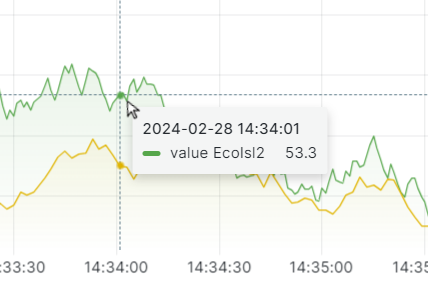
\includegraphics[width=8cm]{../Images/ManualeUtente/Light/dettaglio_time_series_light_bordo.png}}
    \caption{Grafico a linee}
    \label{fig:my_label}
\end{figure}

\paragraph{Lista allerte}
Il pannello contenente la lista degli alert mostra le notifiche delle avvertenze che i sensori hanno riscontrato. Per ciascuna notifica è possibile visualizzare il tipo di avviso, il tempo trascorso dall'attivazione dell'avviso e le istanze coinvolte. \\
Tramite il menu a tendina dedicato a ciascuna notifica, l'utente potrà visualizzare i dettagli dell'avviso.
\begin{figure}[H]
    \centering
    \fbox{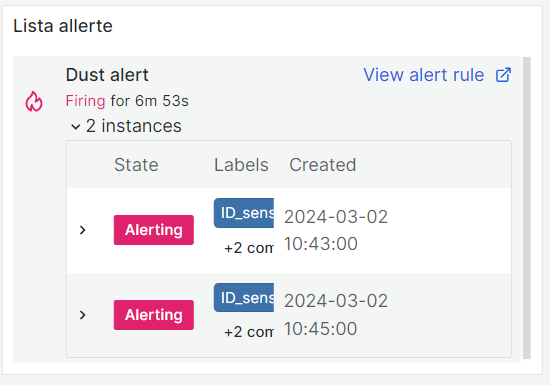
\includegraphics[width=8cm]{../Images/ManualeUtente/Light/alert_panel.png}}
    \caption{Pannello lista allerte}
    \label{fig:my_label}
\end{figure}

\paragraph{Vista tabellare}
\hypertarget{par:tabella}{}
Un grafico tabellare è una rappresentazione visiva dei dati organizzati in forma di tabella, dove le informazioni sono disposte in righe e colonne. Ogni riga della tabella rappresenta una misurazione trasmesse da un \textit{sensore}\textsubscript{\textit{G}}, mentre le colonne rappresentano le diverse variabili o attributi associati. Le celle della tabella possono contenere testo, numeri o altre tipologie di dati, a seconda della natura dei dati rappresentati.
\begin{figure}[H]
    \centering
    \fbox{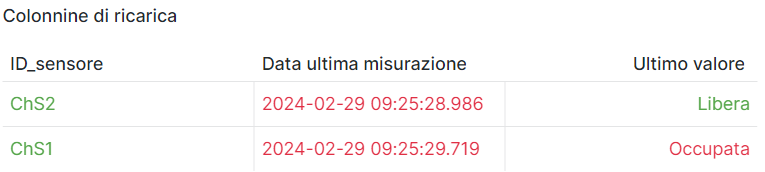
\includegraphics[width=8cm]{../Images/ManualeUtente/Light/vista_tabellare.png}}
    \caption{Vista tabellare}
    \label{fig:my_label}
\end{figure}

\paragraph{Grafico a quadrante}
\hypertarget{par:grafico_quadrante}{}
I grafici a quadrante, noti anche come \textit{gauge}, consentono di visualizzare un singolo valore all'interno di un intervallo specifico. 

\begin{figure}[H]
    \centering
    \fbox{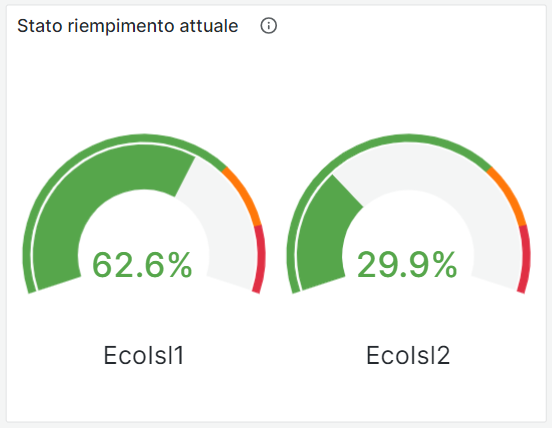
\includegraphics[width=6cm]{../Images/ManualeUtente/Light/gauge_light.png}}
    \caption{Grafico a quadrante}
    \label{fig:my_label}
\end{figure}


\paragraph{Grafico visualizzazione statistiche}
\hypertarget{par:visu_stat}{}
Questa tipologia di grafico consente una visualizzazione chiara e intuitiva dei dati numerici derivati da calcoli ed aggregazioni effettuate sulle misurazioni ottenute dai sensori. 
\begin{figure}[H]
    \centering
    \fbox{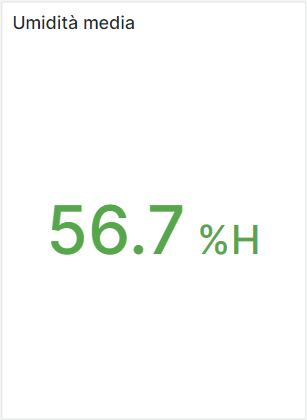
\includegraphics[width=4cm]{../Images/ManualeUtente/Light/stats.png}}
    \caption{Grafico visualizzazione statistiche}
    \label{fig:my_label}
\end{figure}


\subsubsection{Gestione variabili dei grafici}
\hypertarget{par:gestione_variabili_panel}{}
La nostra \textit{piattaforma}\textsubscript{\textit{G}} consente all'utente di gestire di quali sensori visualizzare le misurazioni. Attraverso la selezione delle variabili presenti nella \textit{dashboard}\textsubscript{\textit{G}}, è possibile aggiungere o rimuovere la visualizzazione dei dati relativi ad uno o più sensori, offrendo all'utente la possibilità di personalizzare la propria esperienza di utilizzo. 
\begin{figure}[H]
    \centering
    \fbox{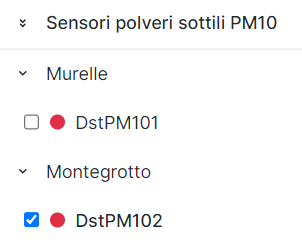
\includegraphics[width=6cm]{../Images/ManualeUtente/Light/variabili_base.png}}
    \caption{pannello variabili dei grafici}
    \label{fig:my_label}
\end{figure}


\subsection{Gruppi di pannelli in dettaglio}
I gruppi di pannelli sono stati progettati per offrire agli utenti una visione completa e dettagliata di un aspetto specifico della città. Ogni gruppo è composto da una serie di pannelli che collaborano per presentare informazioni relative a una singola categoria di dati, come temperatura, umidità, presenza di polveri sottili e altre metriche pertinenti. 

Questi pannelli sono appositamente configurati per essere interattivi e fornire agli utenti dettagli in risposta alle azioni eseguite.
 \\
\subsubsection{City Manager}
Il gruppo di pannelli "City Manager" è stato appositamente concepito per offrire agli utenti una panoramica dettagliata e completa delle informazioni relative alla città. Questo insieme di pannelli è stato progettato con l'obiettivo di fornire una visione esaustiva e immediata dello stato attuale del contesto urbano. \\
Il gruppo è composto da quattro pannelli principali:
\begin{itemize}
    \item \textbf{Pannello di selezione delle celle}: consente agli utenti di selezionare le variabili inerenti alle celle della città affinché il gruppo di pannelli possa visualizzare le informazioni corrispondenti;
    \item \textbf{Mappa dei sensori}: visualizza la posizione dei sensori desiderati nella città;
    \item \textbf{Punteggio di salute}: visualizza il punteggio di salute della città, generato dal calcolo di un indice di qualità delle misurazioni effettuate dai sensori;
    \item \textbf{Lista delle avvertenze}: visualizza le avvertenze relative alla città. Queste avvertenze sono generate dal \textit{sistema}\textsubscript{\textit{G}} in base alle misurazioni effettuate dai sensori e sono visualizzate in tempo reale.
\end{itemize}
\begin{figure}[H]
    \centering
    \fbox{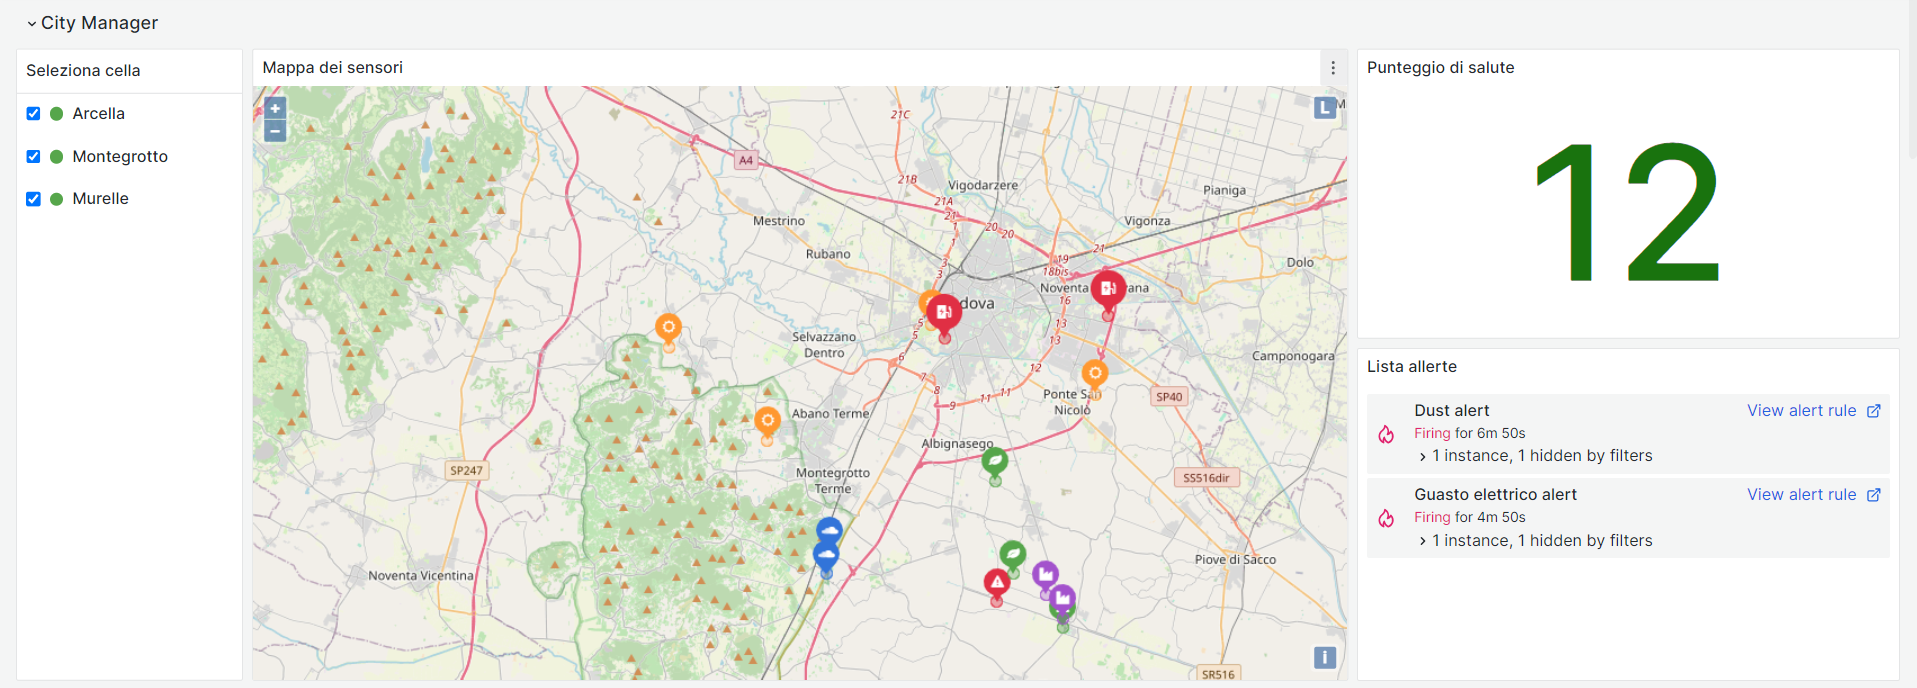
\includegraphics[width=15cm]{../Images/ManualeUtente/Light/gruppo_pannelli_city_manager.png}}
    \caption{Gruppo di pannelli "City Manager"}
    \label{fig:my_label}
\end{figure} 


\subsubsection{Temperatura, Umidità, Polveri sottili}
I gruppi di pannelli "Temperatura", "Umidità" e "Polveri sottili" hanno una struttura simile. Per facilità di comprensione, verrà descritto solo il gruppo di pannelli "Temperatura" ma le stesse informazioni si applicano anche agli altri due gruppi. \\ 
Il gruppo di pannelli "Temperatura" è composto da tre pannelli:
\begin{itemize}
    \item \textbf{Pannello di selezione dei sensori}: consente agli utenti di selezionare i sensori desiderati affinché il gruppo di pannelli possa visualizzare le informazioni corrispondenti;
    \item \textbf{Grafico a linee}: visualizza la temperatura rilevata dai sensori selezionati tramite un grafico a linee descritto nel paragrafo  ~\hyperlink{par:grafico_linee}{\S 3.2.3 - Grafico a linee};
    \item \textbf{Temperatura media}: visualizza la temperatura media rilevata dai sensori selezionati in un determinato intervallo di tempo. La temperatura media viene mostrata all'utente attraverso un grafico "visualizzazione statistiche" come descritto nel paragrafo ~\hyperlink{par:visu_stat}{\S 3.2.3 - Grafico visualizzazione statistiche} e attraverso un valore numerico.
\end{itemize}
\begin{figure}[H]
    \centering
    \fbox{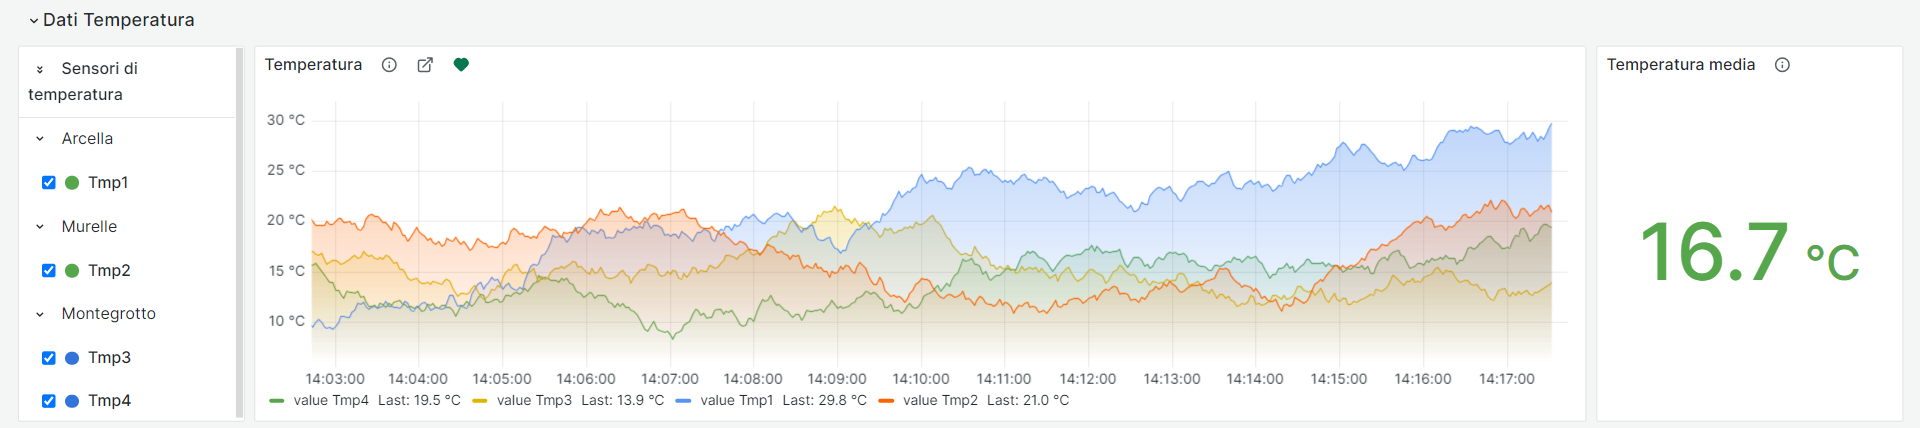
\includegraphics[width=15cm]{../Images/ManualeUtente/Light/gruppo_pannelli_temperatura.png}}
    \caption{Gruppo di pannelli "Temperatura"}
    \label{fig:my_label}
\end{figure}

\subsubsection{Isole ecologiche}
Il gruppo di pannelli "Isole ecologiche" è stato progettato per fornire una visione completa delle informazioni relative alle isole ecologiche. \\
Questo gruppo di pannelli differisce dagli altri descritti sopra in quanto al posto della visualizzazione della temperatura media è presente un grafico a quadrante come descritto nel paragrafo ~\hyperlink{par:grafico_quadrante}{\S 3.2.3 - Grafico a quadrante} che visualizza la percentuale di riempimento delle isole ecologiche. \\
\begin{figure}[H]
    \centering
    \fbox{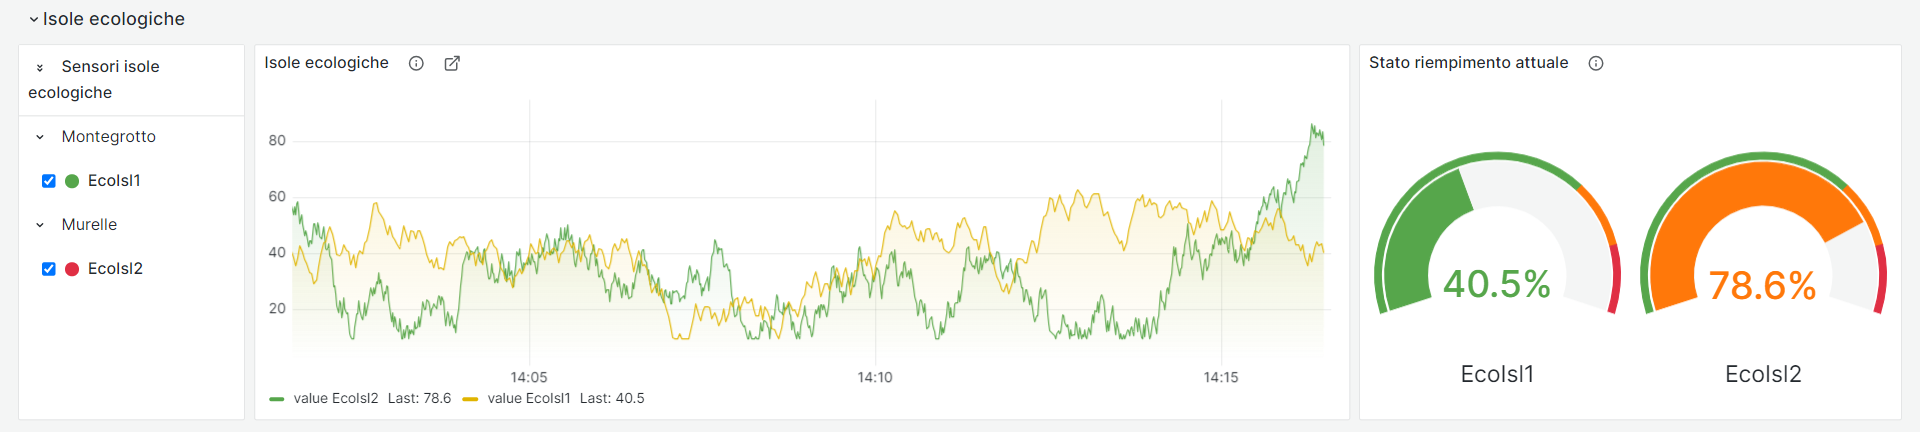
\includegraphics[width=15cm]{../Images/ManualeUtente/Light/gruppo_pannelli_isole.png}}
    \caption{Gruppo di pannelli "Isole ecologiche"}
    \label{fig:my_label}
\end{figure}


\subsubsection{Presenza acqua, Colonnine di ricarica, Guasti elettrici}
I gruppi di pannelli "Presenza acqua", "Colonnine di ricarica" e "Guasti elettrici" hanno una struttura simile. Per facilità di comprensione, verrà descritto solo il gruppo di pannelli "Presenza acqua" ma le stesse informazioni si applicano anche agli altri due gruppi. \\
Il gruppo "Presenza acqua" è composto da quattro pannelli:
\begin{itemize}
    \item \textbf{Sensori presenza acqua}: consente agli utenti di selezionare le variabili (descritte in dettaglio nella sezione ~\hyperlink{par:gestione_variabili_panel}{\S3.2.4}) relative ai sensori desiderati affinché il gruppo di pannelli possa visualizzare le informazioni corrispondenti;
    \item \textbf{Sensori di soglia non attivi}: visualizza i sensori di soglia non attivi tramite un pannello di tipo "visualizzazione statistiche" come descritto nel paragrafo ~\hyperlink{par:visu_stat}{\S 3.2.3 - Grafico visualizzazione statistiche};
    \item \textbf{Sensori di soglia attivi}: visualizza i sensori di soglia attivi tramite un pannello di tipo "visualizzazione statistiche" come descritto nel paragrafo ~\hyperlink{par:visu_stat}{\S 3.2.3 - Grafico visualizzazione statistiche};
    \item \textbf{Sensori di livello acqua}: visualizza i sensori di livello dell'acqua in tabella tramite un pannello di tipo "vista tabellare" come descritto nel paragrafo ~\hyperlink{par:tabella}{\S3.2.3 - Vista tabellare}.
\end{itemize}
\begin{figure}[H]
    \centering
    \fbox{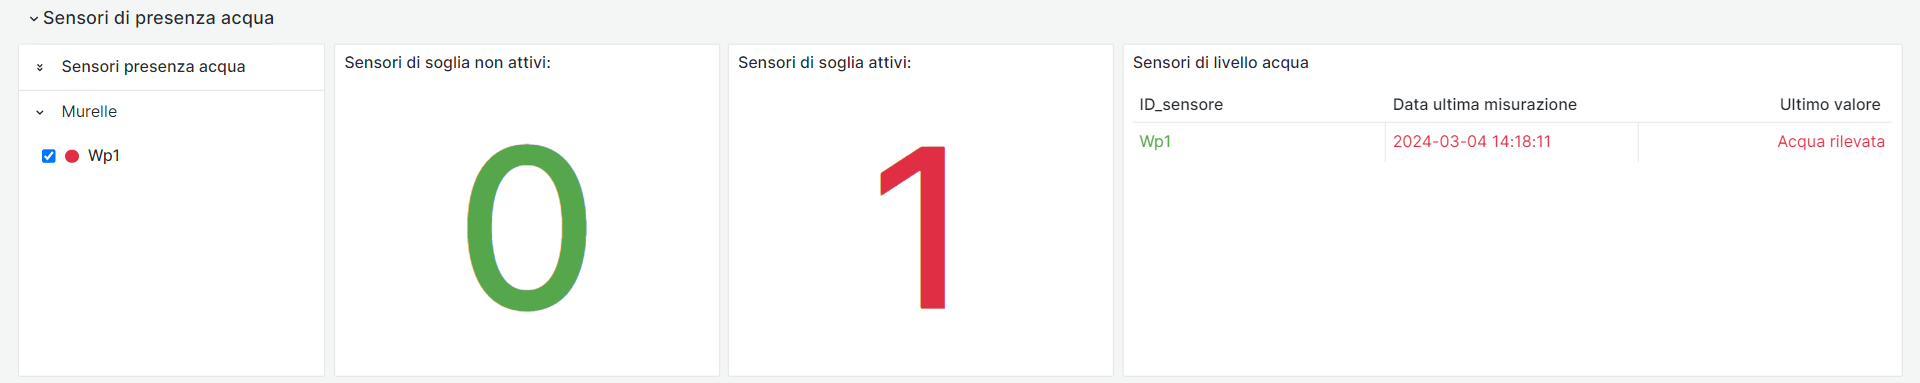
\includegraphics[width=15cm]{../Images/ManualeUtente/Light/gruppo_pannelli_presenza_acqua.png}}
    \caption{Gruppo di pannelli "Presenza acqua"}
    \label{fig:my_label}
\end{figure}

\subsubsection{Minimizzare e massimizzare i gruppi di pannelli}
Ogni gruppo di pannelli può essere minimizzato o massimizzato. Per minimizzare un gruppo di pannelli, l'utente deve fare clic sul nome del gruppo di pannelli o sulla freccetta posta vicino a esso. Per tornare alla visualizzazione massimizzata, l'utente deve fare nuovamente clic sul nome del gruppo di pannelli o sulla freccetta. \\
\begin{figure}[H]
    \centering
    \fbox{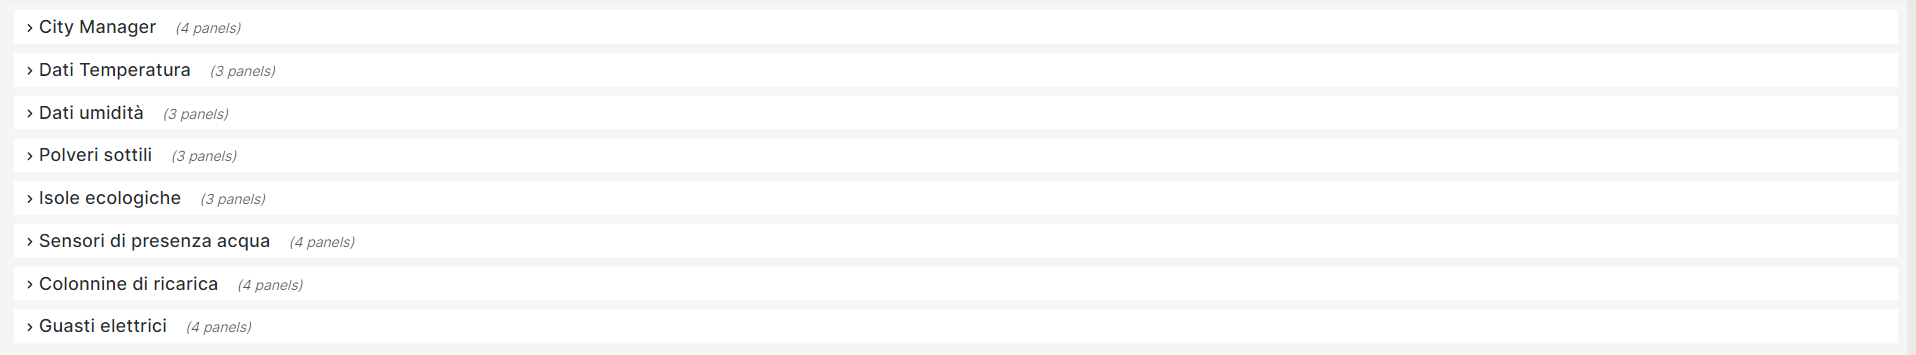
\includegraphics[width=13cm]{../Images/ManualeUtente/Light/gruppo_pannelli_chiusi.png}}
    \caption{Gruppo di pannelli minimizzati}
    \label{fig:my_label}
\end{figure}



\subsection{Dashboard dettagliate}
\subsubsection{Accesso alle dashboard dettagliate}
Cliccando su un bottone posto in ciascun grafico a linee nei gruppi di pannelli, l'utente verrà reindirizzato in una \textit{dashboard}\textsubscript{\textit{G}} contenente i dettagli relativi al gruppo selezionato. 
\begin{figure}[H]
    \centering
    \fbox{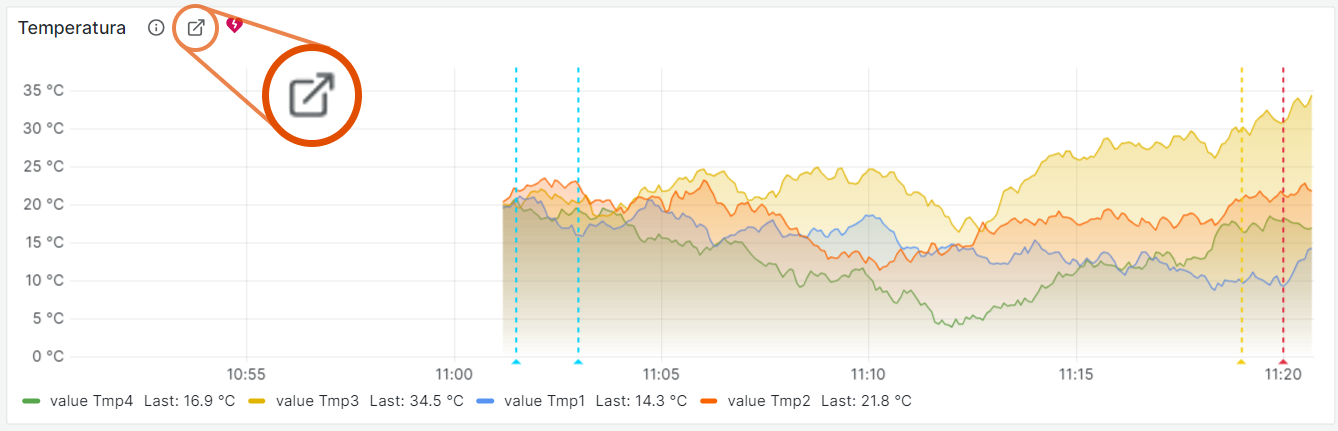
\includegraphics[width=15cm]{../Images/ManualeUtente/Light/temperature_graph_dashboard_dettaglio_alert.png}}
    \caption{Accesso alle dashboard dettagliate}
    \label{fig:my_label}
\end{figure}

\subsubsection{Zoom in Dashboard}
La \textit{dashboard}\textsubscript{\textit{G}} "Zoom in Dashboard" rappresenta il cruscotto verso cui gli utenti sono reindirizzati dopo aver cliccato su un bottone di un gruppo di pannelli. Questa \textit{dashboard}\textsubscript{\textit{G}} è progettata per mostrare in dettaglio le informazioni relative al gruppo di pannelli selezionato, adattando le \textit{query}\textsubscript{\textit{G}} dei vari pannelli per visualizzare esclusivamente i dati pertinenti al gruppo scelto. 
\begin{figure}[H]
    \centering
    \fbox{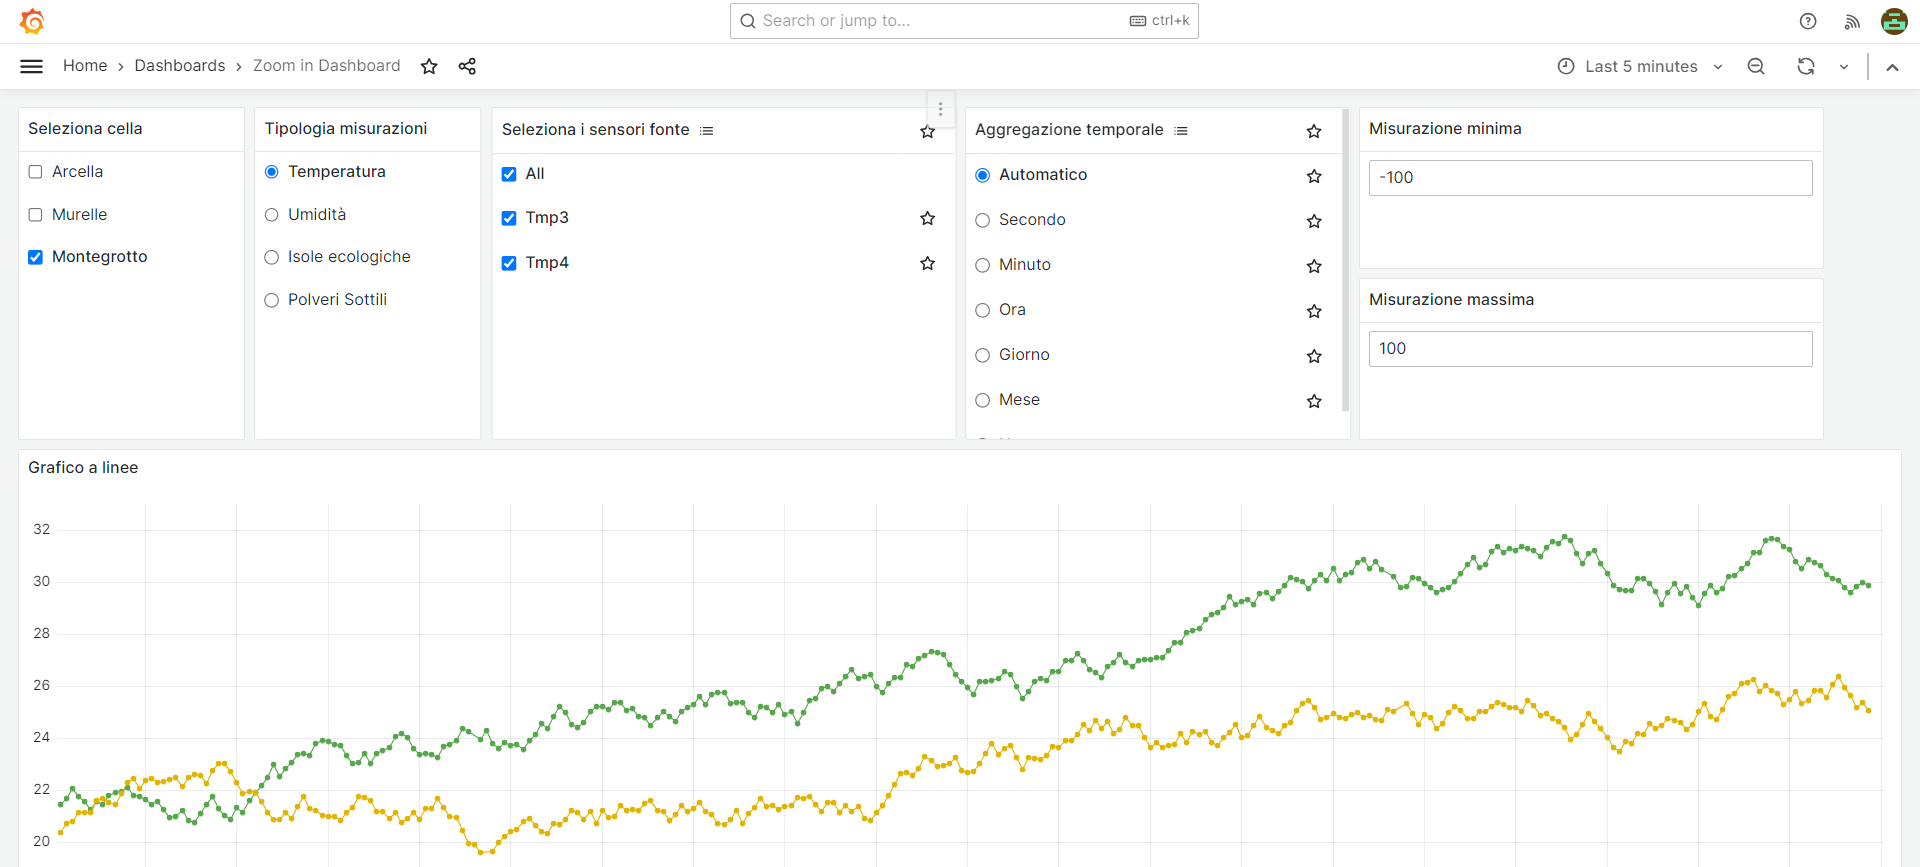
\includegraphics[width=15cm]{../Images/ManualeUtente/Light/dashboard_zoom_in.png}}
    \caption{Dashboard "Zoom in Dashboard"}
    \label{fig:my_label}
\end{figure}

\paragraph{Variabili di ricerca}

La \textit{dashboard}\textsubscript{\textit{G}} "Zoom in Dashboard" offre all'utente la possibilità di personalizzare la visualizzazione dei dati attraverso la modifica dinamica delle variabili di ricerca. Questa flessibilità consente agli utenti di adattare le \textit{query}\textsubscript{\textit{G}} dei grafici in tempo reale alle loro specifiche esigenze, selezionando e visualizzando solo i dati pertinenti.\\
Le variabili offriranno la possibilità di visualizzare i dati in base a diversi parametri, tra cui:
\begin{itemize}
    \item le suddivisioni territoriali delle città;
    \item le tipologie specifiche dei sensori;
    \item il codice univoco attribuito ai singoli sensori;
    \item le diverse aggregazioni temporali applicate ai dati;
    \item il valore massimo e il valore minimo che una misurazione può assumere.
\end{itemize}
\begin{figure}[H]
    \centering
    \fbox{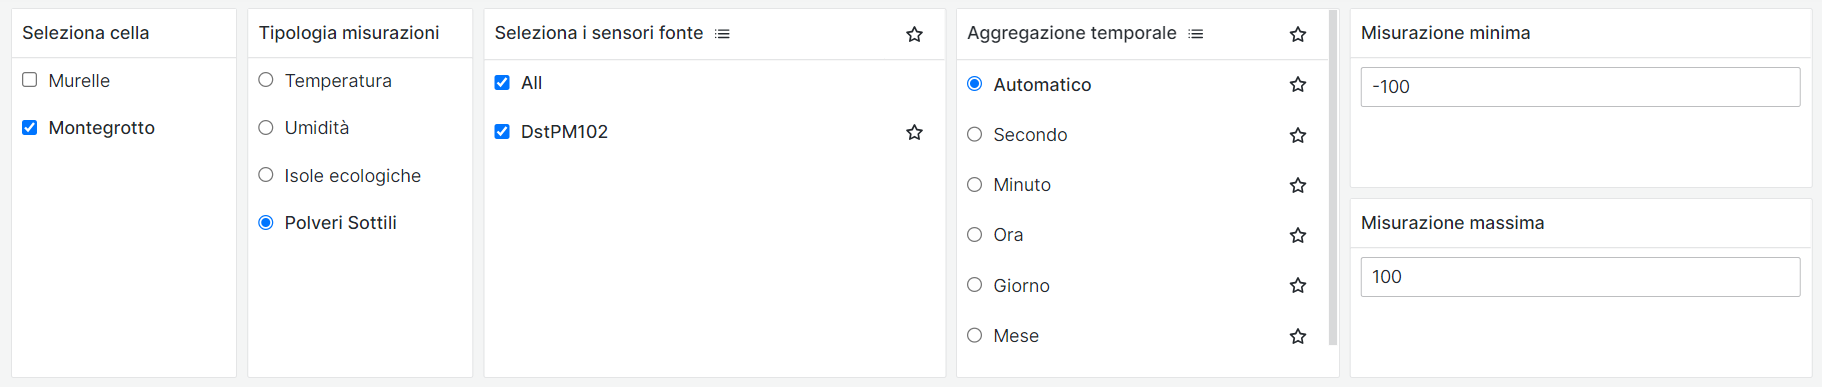
\includegraphics[width=15cm]{../Images/ManualeUtente/Light/variabili_dettaglio_zoom_in.png}}
    \caption{Variabili di ricerca}
    \label{fig:my_label}
\end{figure}




\subsection{Profilo utente}
La schermata del profilo utente è accessibile cliccando sull'icona dell'utente posizionata in alto a destra nella barra degli strumenti, come specificato nel paragrafo ~\S\hyperlink{par:pulsante_profilo}{3.2.1 - Pulsante profilo utente}. Da questa schermata, gli utenti possono visualizzare e modificare le proprie informazioni personali, nonché accedere alle preferenze dell'utente per apportare eventuali modifiche. \\
La schermata del profilo utente è composta da tre schede principali:
\begin{itemize}
    \item Profile;
    \item Notification history;
    \item Change password.
\end{itemize}
\begin{figure}[H]
    \centering
    \fbox{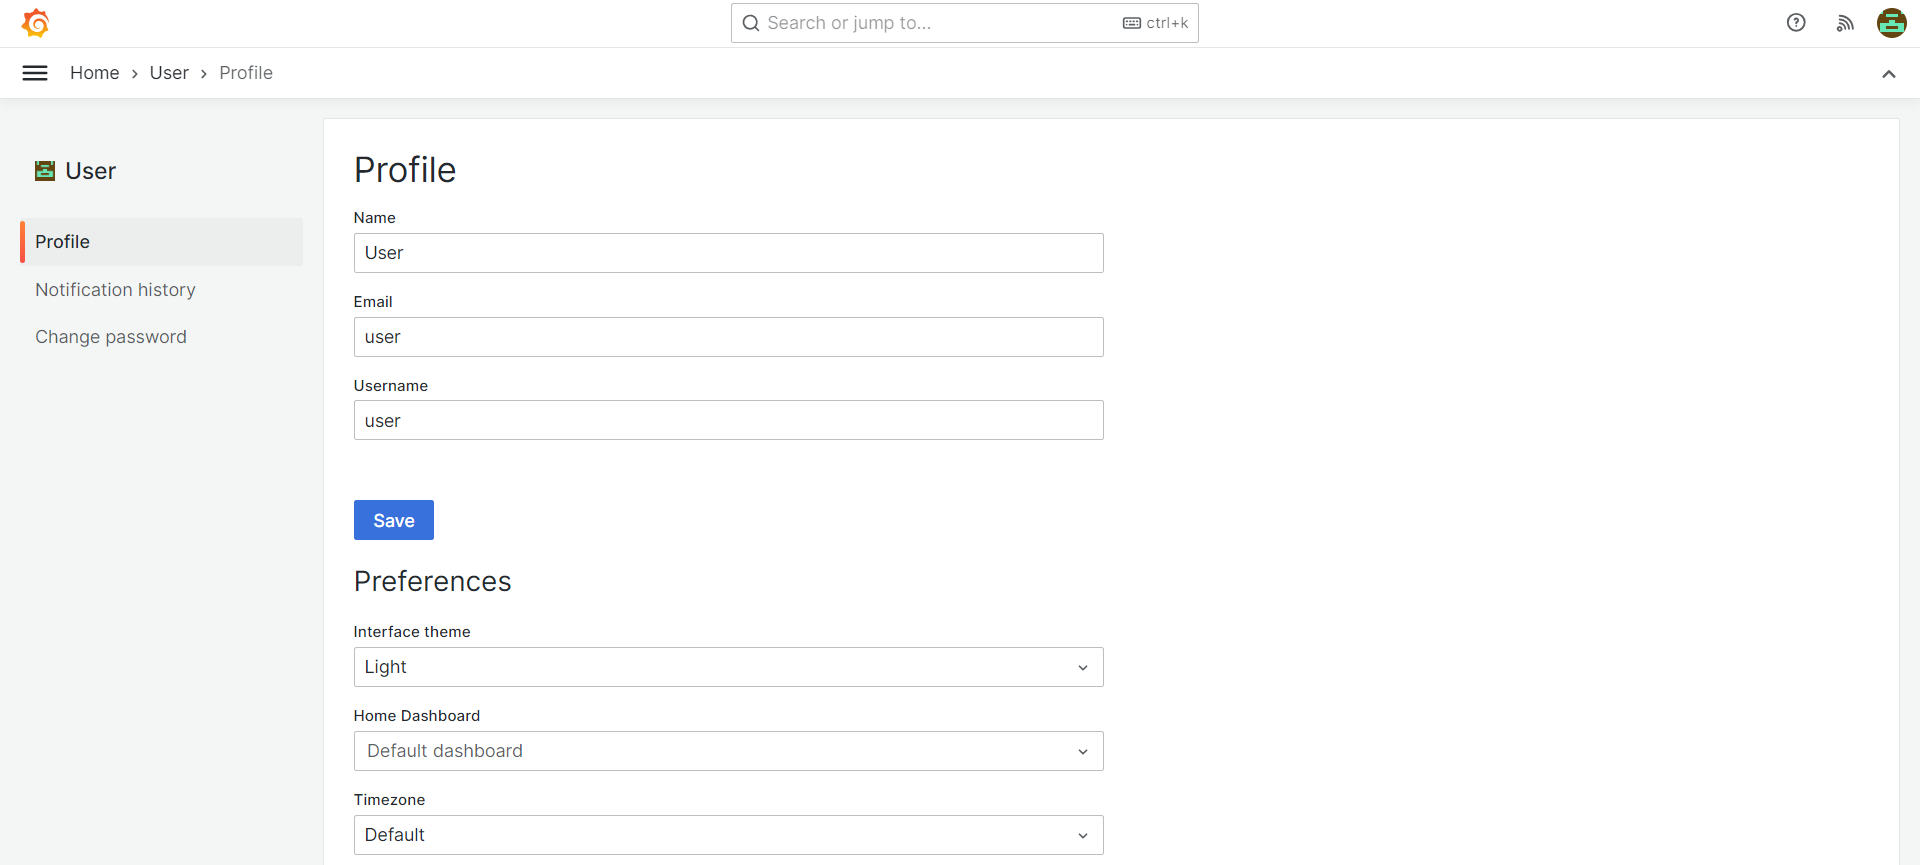
\includegraphics[width=16cm]{../Images/ManualeUtente/Light/schermata_profilo_utente.png}}
    \caption{Schermata del profilo utente}
    \label{fig:my_label}
\end{figure} 

\subsubsection{Profile}
La schermata dedicata al profilo utente consente di visualizzare e modificare le informazioni personali dell'utente. In particolare è possibile visualizzare e modificare nome, email, ed username. Una volta apportate le modifiche desiderate, è possibile confermarle cliccando sul pulsante "Save". \\
Sono presenti altre tre sottosezioni:
\begin{itemize}
    \item Preferences;
    \item Organizations;
    \item Sessions.
\end{itemize}
\paragraph{Preferences}
La sezione "Preferences" consente di modificare le seguenti preferenze:
\begin{itemize}
    \item Tema dell'interfaccia;
    \item \textit{Dashboard}\textsubscript{\textit{G}} predefinita (Home \textit{dashboard}\textsubscript{\textit{G}});
    \item Fuso orario;
    \item Inizio della settimana;
    \item Lingua;
\end{itemize}
Una volta modificata la scelta tramite un pratico menù a tendina, è possibile confermare le modifiche cliccando sul pulsante "Save". \\
\paragraph{Organizations}
La sezione "Organizations" consente di visualizzare le organizzazioni a cui l'utente appartiene. Per ogni organizzazione è possibile visualizzare il nome e il ruolo dell'utente all'interno di essa.
\begin{figure}[H]
    \centering
    \fbox{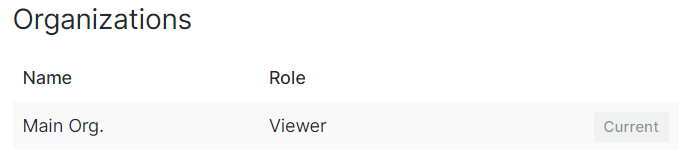
\includegraphics[width=10cm]{../Images/ManualeUtente/Light/profile_organizations.png}}
    \caption{Profilo utente sezione "Organizzazioni"}
    \label{fig:my_label}
\end{figure}
\paragraph{Sessions}
La sezione "Sessions" consente di visualizzare le sessioni attive dell'utente. Per ciascuna sessione è possibile visualizzare la data e l'ora dell'ultimo accesso, l'indirizzo \textit{IP}\textsubscript{\textit{G}}, nonché il \textit{browser}\textsubscript{\textit{G}} e il \textit{sistema}\textsubscript{\textit{G}} operativo utilizzati. Attraverso un pulsante dedicato, è possibile terminare la sessione desiderata.
\begin{figure}[H]
    \centering
    \fbox{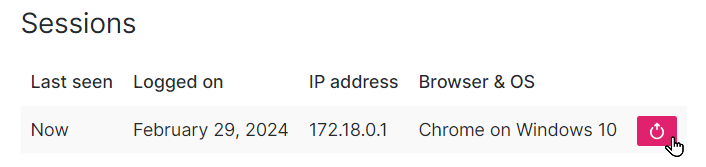
\includegraphics[width=10.5cm]{../Images/ManualeUtente/Light/profile_sessions.png}}
    \caption{Profilo utente sezione "Sessioni"}
    \label{fig:my_label}
\end{figure}

\subsubsection{Notification history}
La schermata "Notification history" consente di visualizzare la cronologia delle notifiche degli errori o delle avvertenze. Per ciascuna notifica è possibile visualizzare la data e l'ora, il tipo di notifica e, se presente il messaggio corrispondente.
\begin{figure}[H]
    \centering
    \fbox{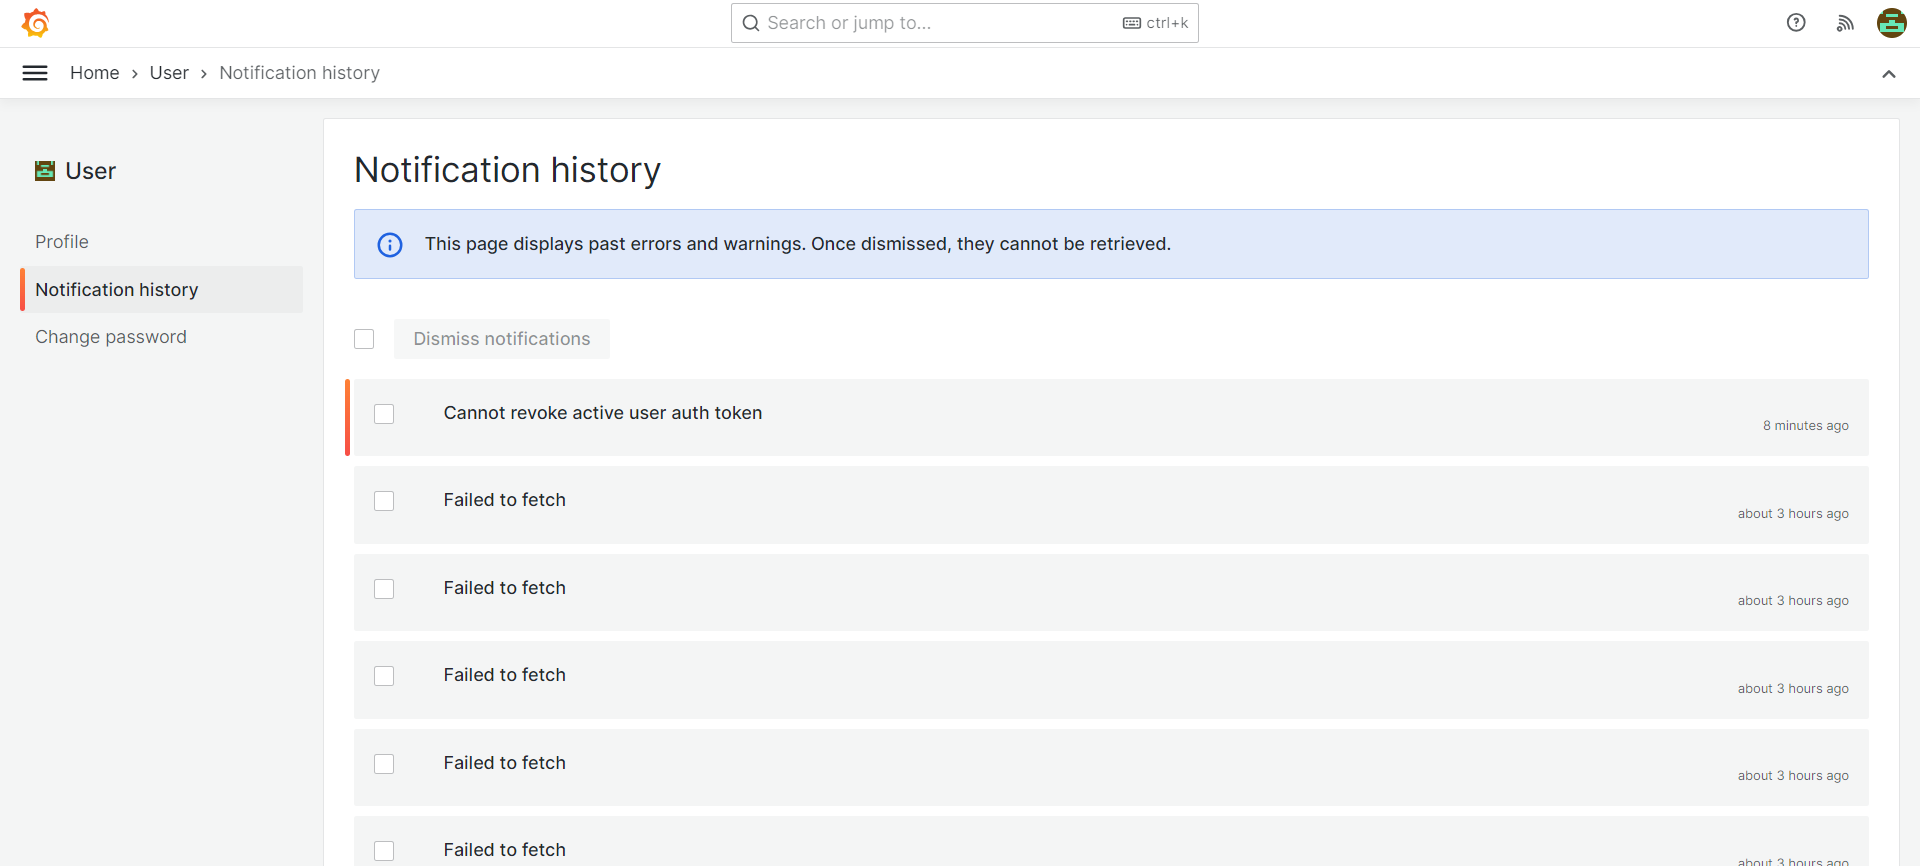
\includegraphics[width=16cm]{../Images/ManualeUtente/Light/notifications_history.png}}
    \caption{Schermata "Cronologia delle notifiche"}
    \label{fig:my_label}
\end{figure}
È possibile selezionare una o più notifiche e cliccando sul pulsante "Dismiss notifications" è possibile eliminare le notifiche selezionate (una volta cancellate non sarà più possibile recuperarle).  
\begin{figure}[H]
    \centering
    \fbox{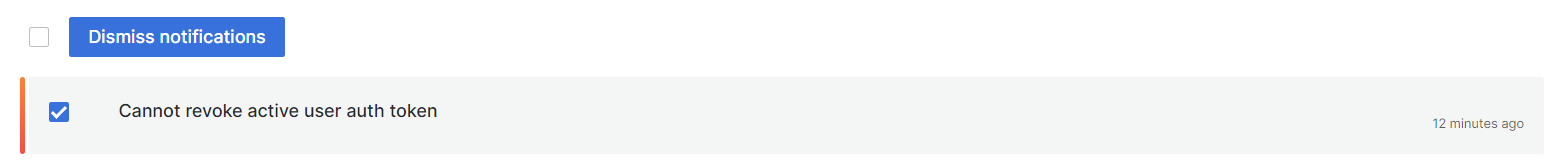
\includegraphics[width=12cm]{../Images/ManualeUtente/Light/dismiss_notificaitions.png}}
    \caption{Cancellare le notifiche}
    \label{fig:my_label}
\end{figure}

\subsubsection{Change password}
La schermata "Change password" consente di modificare la password dell'utente. Per modificare la password è necessario inserire la password corrente, la nuova password e confermare la nuova password. Una volta inserite le informazioni richieste, è possibile confermare le modifiche cliccando sul pulsante "Change Password" o, in alternativa, annullare le modifiche cliccando sul pulsante "Cancel". 
\begin{figure}[H]
    \centering
    \fbox{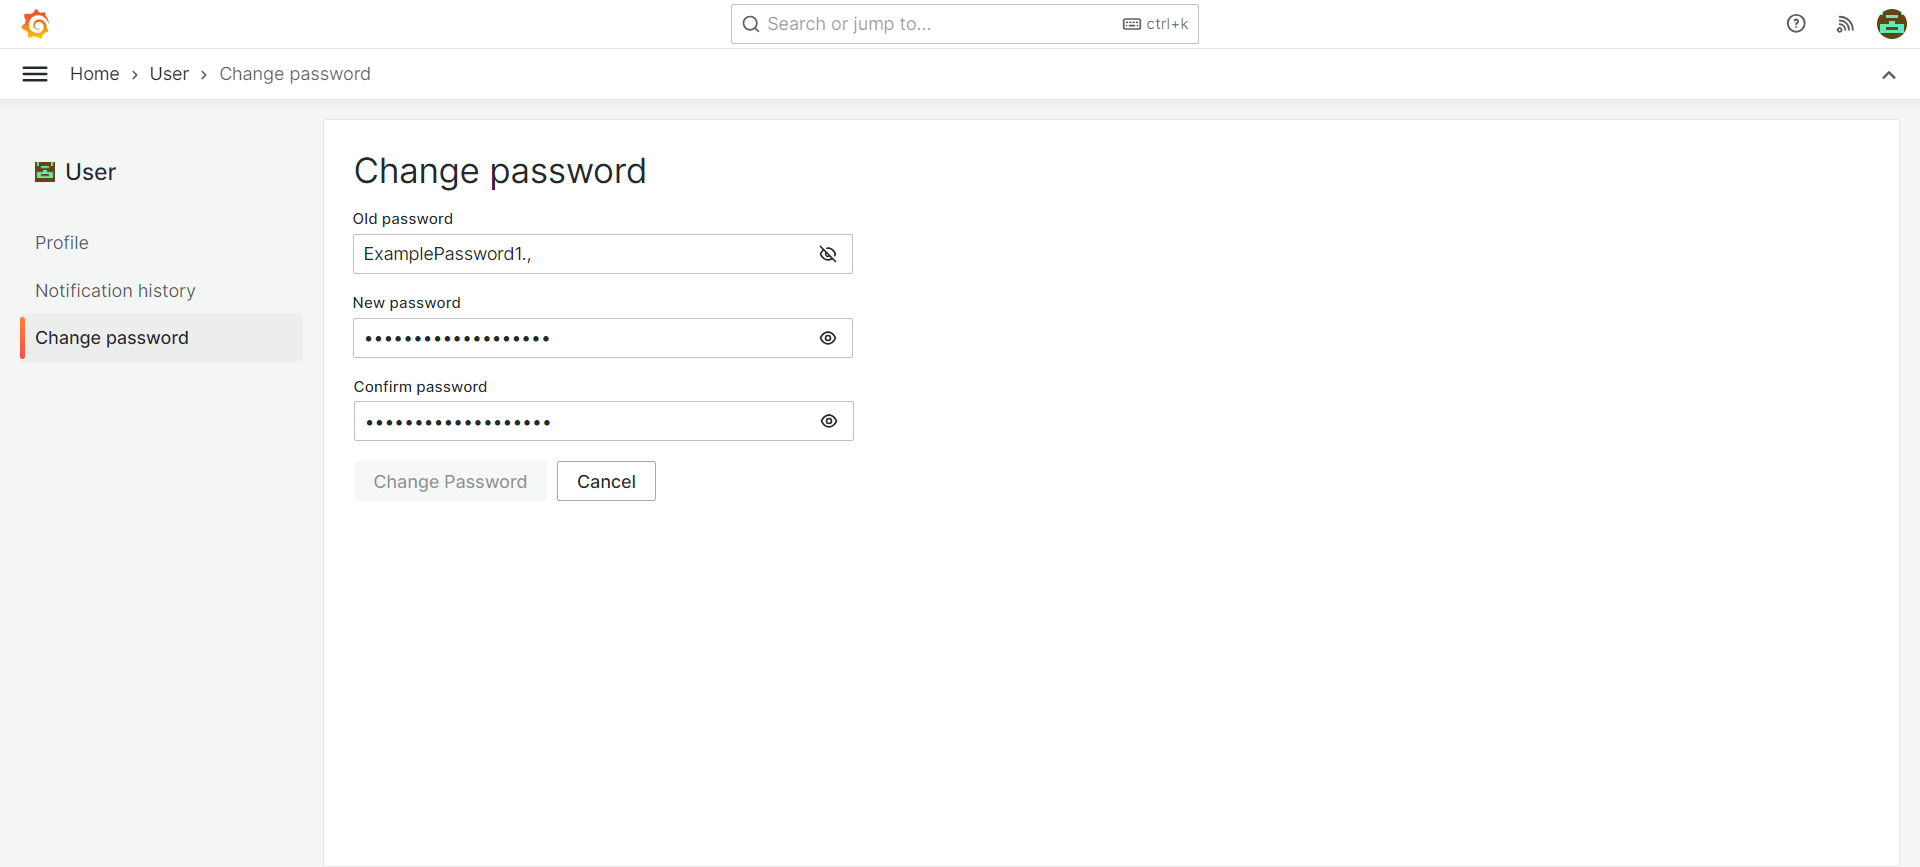
\includegraphics[width=16cm]{../Images/ManualeUtente/Light/cambia_password.png}}
    \caption{Schermata "Cambia password"}
    \label{fig:my_label}
\end{figure}
Cliccando sull'icona rappresentante un occhio, è possibile visualizzare la password inserita e, cliccando nuovamente sull'icona, è possibile nascondere la password.
\begin{figure}[H]
    \centering
    \fbox{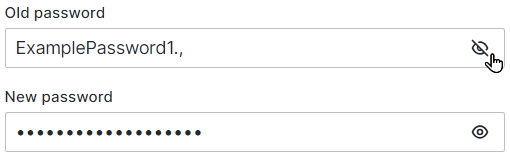
\includegraphics[width=8cm]{../Images/ManualeUtente/Light/visualizza_password.png}}
    \caption{Visualizzare la password inserita}
    \label{fig:my_label}
\end{figure}
\begin{center}
    \textbf{Attenzione}: la password inserita nell'immagine è a puro scopo illustrativo e non rappresenta la password reale dell'utente. \\
\end{center}
 
\subsection{Alert}
Gli alert, conosciuti anche come allarmi, costituiscono notifiche inviate agli utenti per segnalare eventuali problemi o situazioni di criticità rilevate dai sensori.\\
Essi vengono generati in risposta al superamento di una soglia di allarme predefinita da parte di un evento. \\

\subsubsection{Visualizzazione degli Alert}
Gli alert vengono mostrati in un riquadro dedicato nella \textit{dashboard}\textsubscript{\textit{G}} principale, come mostrato nella sotto-sezione relativa alle tipologie dei grafici (\S\ref{subsec:tipologie_grafici}). \\

\paragraph{Alert nei grafici}
In alcuni pannelli è possibile vedere gli alert direttamente nei grafici. In particolare è possibile visualizzare gli alert nei grafici a linee come una linea tratteggiata verticale che indica il punto nel tempo in cui l'alert è stato attivato. \\
\begin{figure}[H]
    \centering
    \fbox{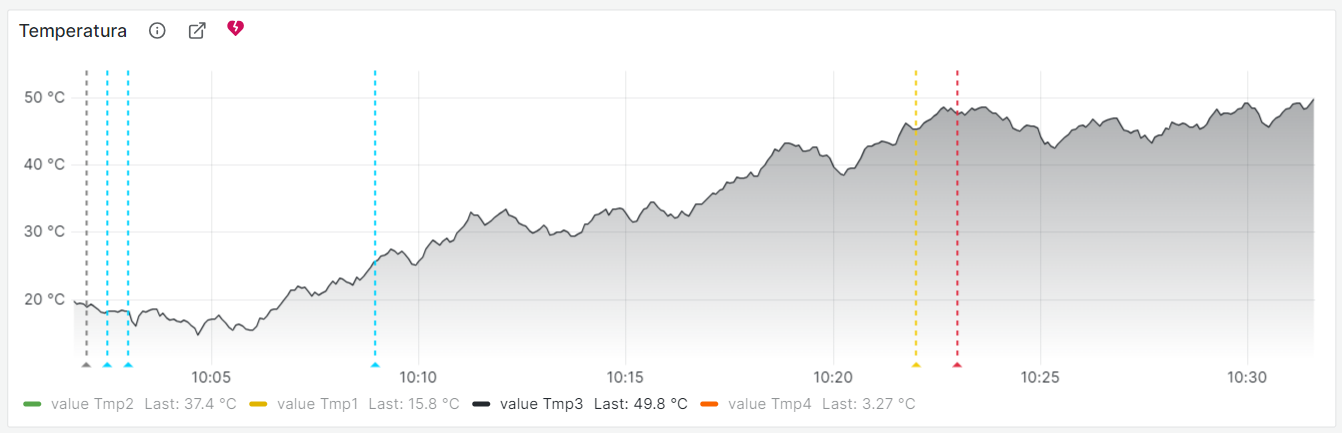
\includegraphics[width=12cm]{../Images/ManualeUtente/Light/panel_singolo_grafico.png}}
    \caption{Esempio di alert in un grafico a linee}
    \label{fig:my_label}
\end{figure}
Come si può notare dall'immagine sopra, in alto a sinistra è presente un'icona a forma di cuore che indica lo stato dell'alert del grafico. Può essere di tre tipi: 

\begin{itemize}
    \item \textbf{Ok}: l'icona rappresenta un cuore intero e non è presente alcuna linea tratteggiata nel grafico; 
    \begin{figure}[H]
        \centering
        \fbox{
\includegraphics[width=4cm]{../Images/ManualeUtente/Light/alert_pannello_cuore_ok.png}}
        \caption{Stato "ok" dell'alert}
        \label{fig:my_label}
    \end{figure}
    \item \textbf{Alert pending}: 
    quando una condizione per l'attivazione dell'avviso è stata soddisfatta, ma il periodo di valutazione dell'avviso non è ancora trascorso. Il periodo di valutazione negli alert è il lasso di tempo durante il quale il \textit{sistema}\textsubscript{\textit{G}} verifica continuamente se una condizione di allarme è soddisfatta.  
    \begin{figure}[H]
        \centering
        \fbox{
\includegraphics[width=4cm]{../Images/ManualeUtente/Light/alert_pannello_cuore_pending.png}}
        \caption{Stato "pending" dell'alert}
        \label{fig:my_label}
    \end{figure}
    \item \textbf{Alert attivo}: quando una condizione di attivazione dell'avviso è stata soddisfatta e il periodo di valutazione dell'avviso è trascorso. Come specificato nel punto precedente, il periodo di valutazione negli alert è il lasso di tempo durante il quale il \textit{sistema}\textsubscript{\textit{G}} verifica continuamente se una condizione di allarme è soddisfatta.   
    \begin{figure}[H]
        \centering
        \fbox{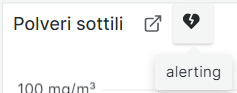
\includegraphics[width=4cm]{../Images/ManualeUtente/Light/alert_pannello_cuore_alerting.png}}
        \caption{Stato "alerting" dell'alert}
        \label{fig:my_label}
    \end{figure}
\end{itemize}

\paragraph{Ricezione notifiche alert}
É reso disponibile agli utenti un server discord dedicato per ricevere le notifiche degli alert in tempo reale. \\


\subsubsection{Server Discord}

\paragraph{Accesso al server Discord}
Qualora l'utente non fosse già iscritto a \textit{Discord}\textsubscript{\textit{G}}, è necessario creare un \textit{account}\textsubscript{\textit{G}} seguendo le istruzioni fornite dal sito ufficiale di \href{https://discord.com/}{Discord}. \\
Per poter accedere al server dedicato, è necessario seguire i seguenti passaggi:
\begin{enumerate}
    \item Accedere al server tramite il \textit{link}\textsubscript{\textit{G}} del server: \href{https://discord.gg/9VZ8me7x}{InnovaCity};
    \item Eseguire l'accesso al proprio \textit{account}\textsubscript{\textit{G}} o, nel caso non se ne fosse in possesso, creare un nuovo \textit{account}\textsubscript{\textit{G}};
    \begin{figure}[H]
        \centering
        \fbox{
\includegraphics[width=9cm]{../Images/ManualeUtente/Light/accesso_discord.png}}
        \caption{Esempio di notifica di un alert su Discord}
        \label{fig:my_label}
    \end{figure}
    \item Una volta entrati nel server, sarà possibile visualizzare le notifiche degli alert in tempo reale nella sezione Informazioni/allerte. 
    \begin{figure}[H]
        \centering
        \fbox{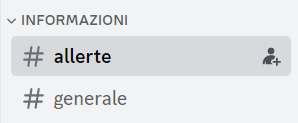
\includegraphics[width=4.5cm]{../Images/ManualeUtente/Light/canale_testuale.png}}
        \caption{Sezione del server Discord dedicata alle notifiche degli alert}    
        \label{fig:my_label}
    \end{figure}
\end{enumerate}

\paragraph{Ricezione delle notifiche su Discord}
Una volta entrati nel server \textit{Discord}\textsubscript{\textit{G}} sarà possibile ricevere le notifiche degli alert in tempo reale. Le notifiche vengono inviate in automatico dal \textit{sistema}\textsubscript{\textit{G}} e sono visibili nella sezione "informazioni/alert" del server \textit{Discord}\textsubscript{\textit{G}}. \\
Gli alert verranno mostrati nel seguente formato:
\begin{figure}[H]
    \centering
    \fbox{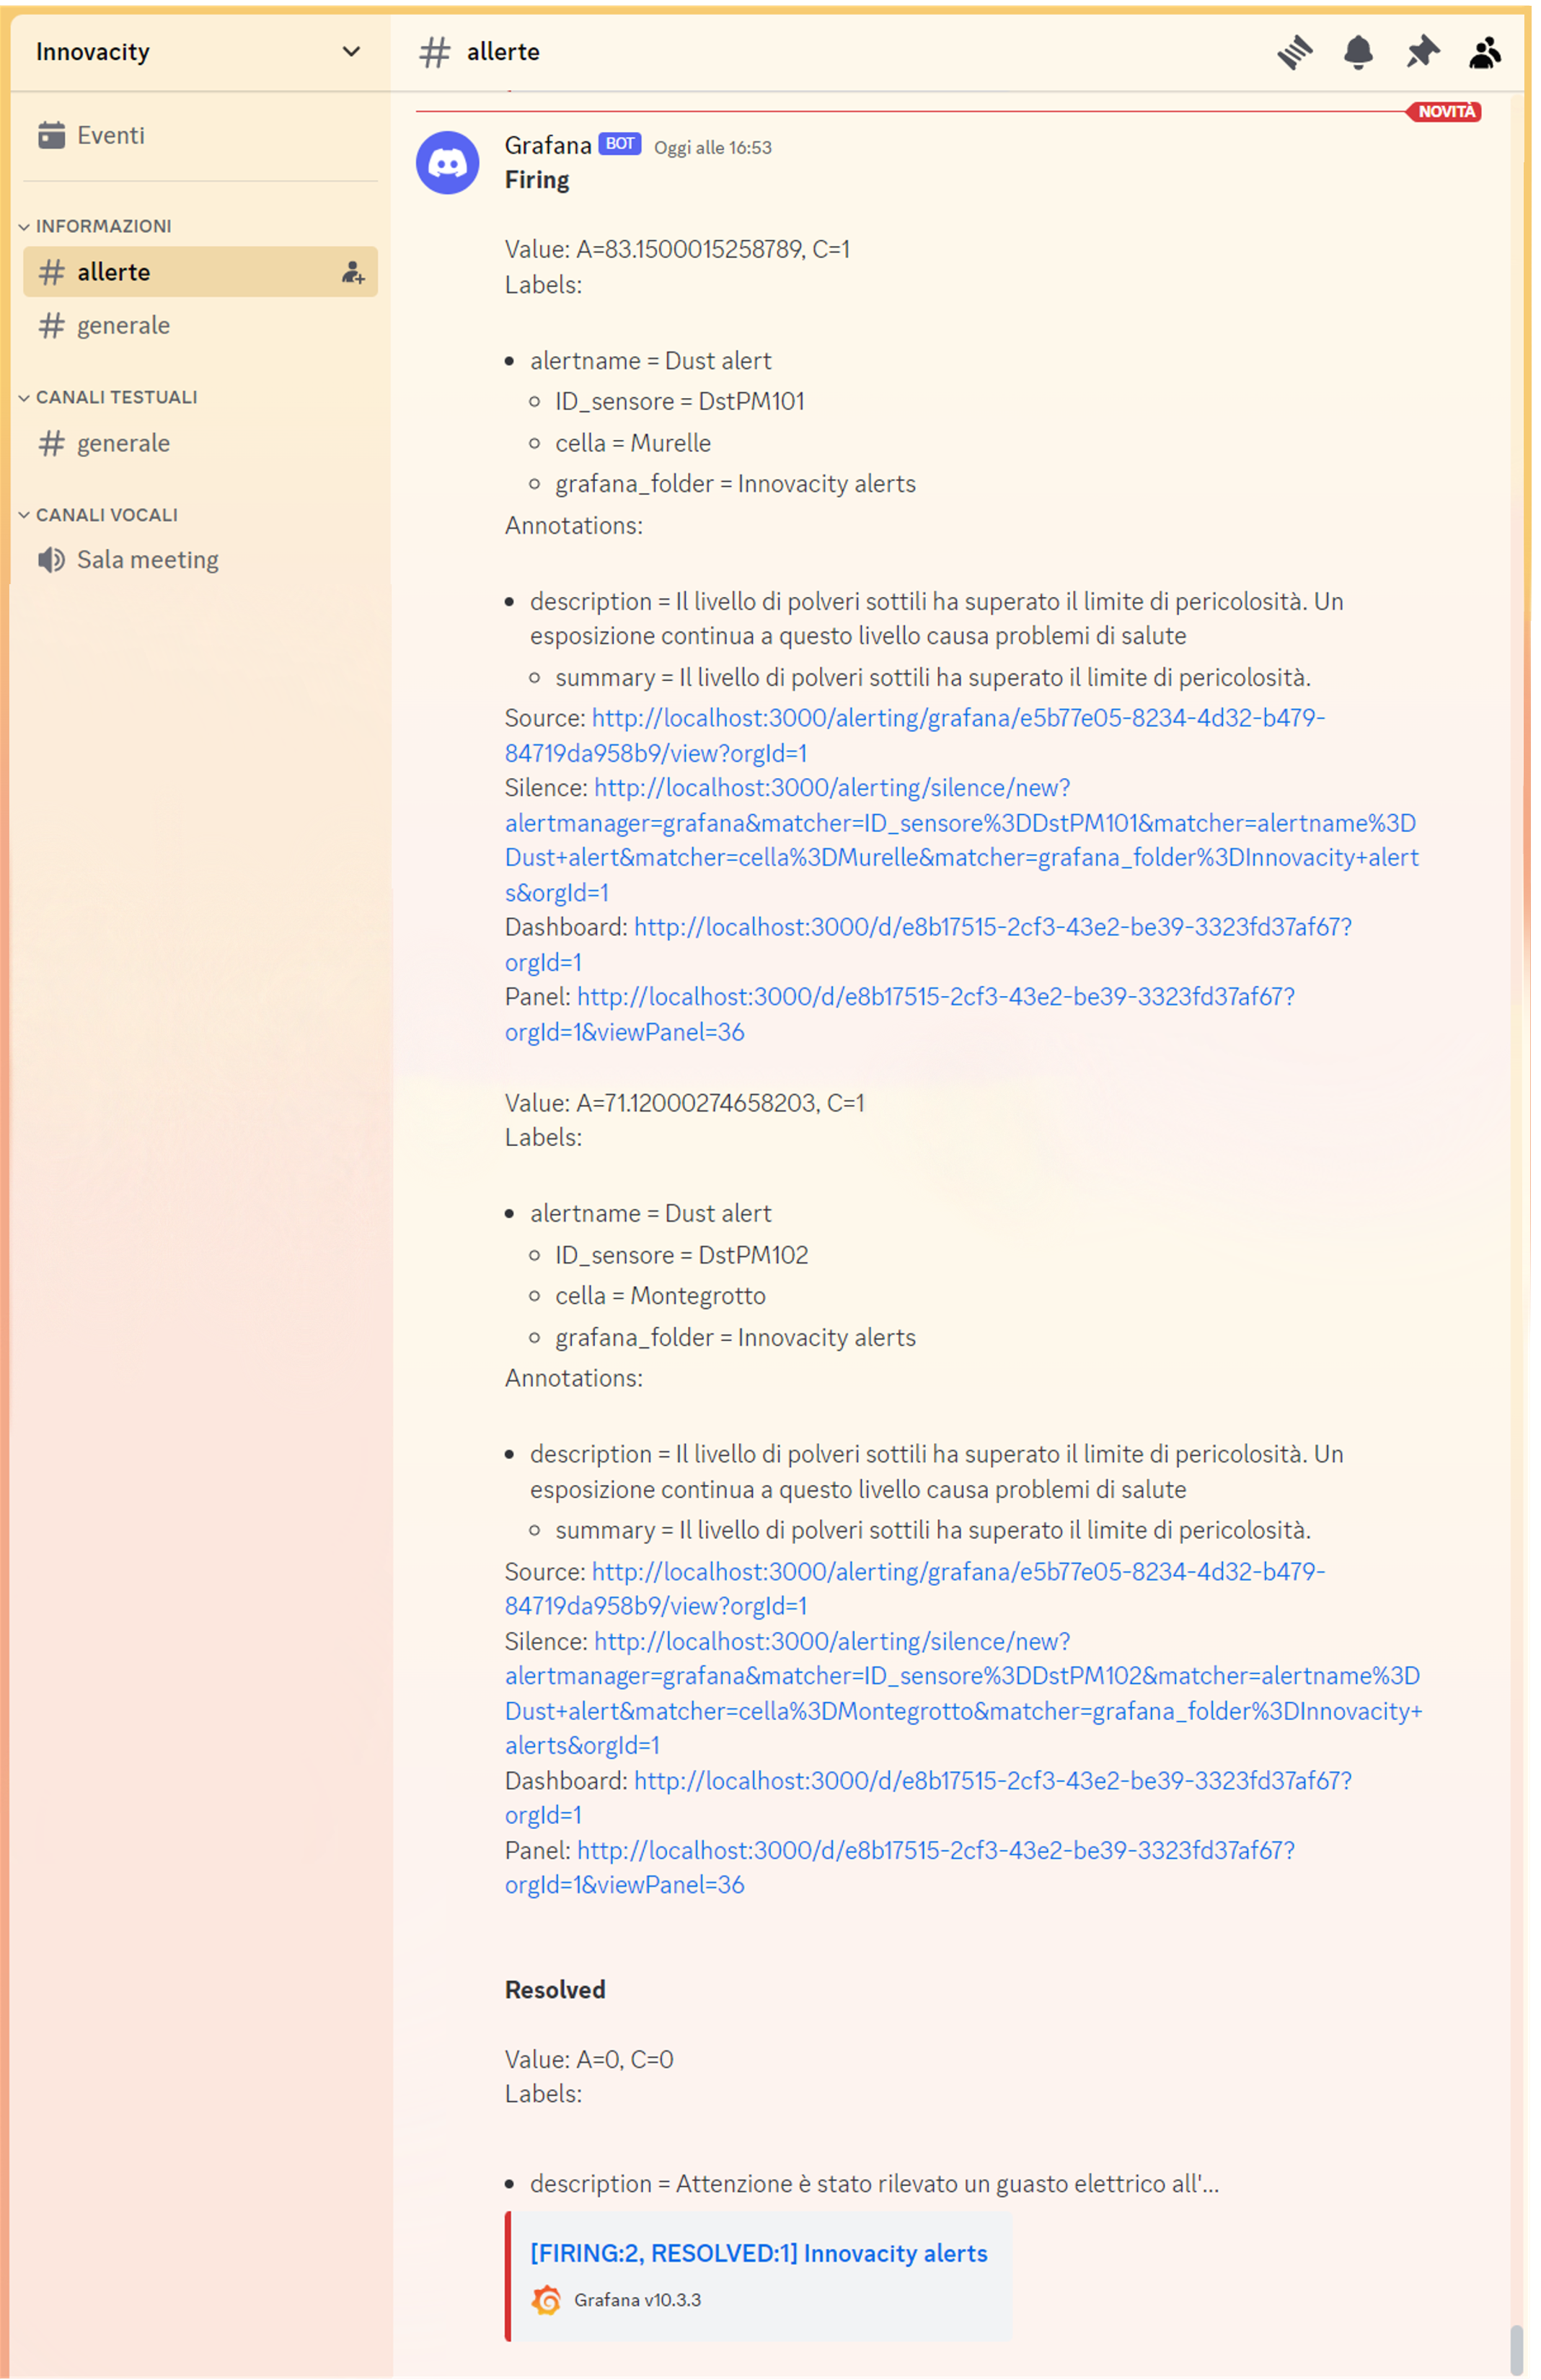
\includegraphics[width=8cm]{../Images/ManualeUtente/Light/discord_notification.png}}
    \caption{Esempio di notifica di un alert su Discord}
    \label{fig:my_label}
\end{figure} 
% \subsection{Riferimenti}
\subsubsection{Riferimenti informativi}
    \begin{itemize}
        \item \href {https://www.math.unipd.it/~tullio/IS-1/2023/Progetto/C6.pdf} {Capitolato d'appalto C6 - InnovaCity }
        \item \href{https://www.math.unipd.it/~tullio/IS-1/2023/Dispense/T4.pdf} {Slide del corso di Ingegneria del Software - Gestione di progetto }
        \item \href{https://www.math.unipd.it/~tullio/IS-1/2023/Dispense/T2.pdf} {Slide del corso di Ingegneria del Software - Ciclo di vita del software }
    \end{itemize}
 
\subsubsection{Riferimenti normativi}
    \begin{itemize}
    \item Norme di progetto
    \item \href {https://www.math.unipd.it/~tullio/IS-1/2023/Dispense/PD2.pdf} {Regolamento del progetto didattico }
    \end{itemize}

\vspace{0.5cm}

\end{document}
